\clearpage

\chapter{SYSTEM ANALYSIS}

System analysis establishes the foundational functional requirements, dataset architecture, exploratory statistical properties, preprocessing transformations, algorithmic mechanics, and deployment feasibility for the automated Medical Specialty Classification system.

The empirical investigation is conducted on the Kaggle Medical Transcriptions (MTSamples) dataset \cite{mtsamples_dataset}, which provides authentic, transcribed clinical dictations across diverse healthcare disciplines. Analyzing this corpus facilitates the development of a clinically sound, computationally lightweight natural language processing pipeline capable of differentiating domain-specific medical vocabulary while remaining suitable for real-time web deployment on standard CPU hardware.

\chapter{Analysis of the dataset}

\chapter{About the dataset}

\chapter{Dataset Overview}
The Kaggle Medical Transcriptions dataset is a curated collection of authentic clinical narratives obtained from MTSamples.com, an open clinical transcription repository created to assist medical transcriptionists and healthcare informatics researchers. The dataset encapsulates a broad spectrum of real-world clinical encounters, ranging from routine consultative histories and physical examinations to highly complex intraoperative surgical summaries.
\begin{itemize}
    \item \textbf{Total Raw Records}: 4,999 clinical transcription reports.
    \item \textbf{Total Attributes}: 6 attributes (1 integer identifier, 4 textual features, and 1 categorical target label).
    \item \textbf{Data Types}: Free-text clinical narratives (\texttt{transcription}), diagnostic abstracts (\texttt{description}), comma-delimited keywords (\texttt{keywords}), procedure titles (\texttt{sample\_name}), and categorical specialty labels (\texttt{medical\_specialty}).
    \item \textbf{Target Attribute}: \texttt{medical\_specialty}, containing 40 nominal medical department categories in the raw distribution.
\end{itemize}

Table \ref{tab:dataset_summary_card} summarizes the fundamental structural characteristics of the raw dataset.

\begin{table}[H]
\centering
\small
\setlength{\tabcolsep}{5pt}
\begin{tabularx}{\linewidth}{|>{\raggedright\arraybackslash}p{3.8cm}|>{\raggedright\arraybackslash}X|}
\hline
\textbf{Property} & \textbf{Description} \\
\hline
\textbf{Dataset Name} & Kaggle Medical Transcriptions (MTSamples) Dataset \\
\hline
\textbf{Source} & Kaggle (\url{https://www.kaggle.com/datasets/tboyle10/medicaltranscriptions}) \\
\hline
\textbf{Total Raw Records} & 4,999 clinical reports \\
\hline
\textbf{Number of Attributes} & 6 fields (\texttt{Unnamed: 0}, \texttt{description}, \texttt{medical\_specialty}, \texttt{sample\_name}, \texttt{transcription}, \texttt{keywords}) \\
\hline
\textbf{Primary Feature Variable} & \texttt{transcription} (Unstructured clinical narrative dictation) \\
\hline
\textbf{Auxiliary Feature Variable} & \texttt{description} (Short diagnostic synopsis) \\
\hline
\textbf{Target Class Variable} & \texttt{medical\_specialty} (40 raw categories; curated to 8 core specialties + 1 Open-Set class) \\
\hline
\textbf{Advantages} & Authentic clinical language; zero missing target labels (100\% labeled); rich multi-specialty terminology \\
\hline
\textbf{Challenges} & Severe category imbalance; missing transcription entries (33 nulls); overlapping administrative document categories \\
\hline
\end{tabularx}
\caption{Characteristics of the Kaggle Medical Transcriptions Dataset}
\label{tab:dataset_summary_card}
\end{table}

\chapter{Attribute Specifications}
The six dataset attributes serve distinct analytical functions:
\begin{enumerate}
    \item \textbf{Record Identifier (\texttt{Unnamed: 0})}: An integer sequence representing the raw tabular row index (range: 0 to 4,998).
    \item \textbf{Clinical Abstract (\texttt{description})}: A concise, one-to-two sentence clinical synopsis summarizing the patient's presenting condition, consultation findings, or surgical objective.
    \item \textbf{Target Medical Specialty (\texttt{medical\_specialty})}: The categorical label designating the medical specialty or departmental division under which the transcription was categorized.
    \item \textbf{Dictation Title (\texttt{sample\_name})}: A brief descriptive title denoting the specific clinical procedure, anatomical site, or encounter type (e.g., ``Coronary Artery Bypass'', ``Colonoscopy'').
    \item \textbf{Primary Clinical Narrative (\texttt{transcription})}: The central predictor feature containing the full, free-text clinical dictation. It details the patient's medical history, physical examination, diagnostic investigations, intraoperative findings, and postoperative care plans.
    \item \textbf{Extracted Keywords (\texttt{keywords})}: Comma-delimited medical keywords and anatomical descriptors indexed from the report.
\end{enumerate}

\chapter{Explore the dataset}

\chapter{Statistical Data Profiling and Null Value Audit}
Exploratory data profiling was conducted using Python data analysis frameworks (\texttt{pandas}, \texttt{numpy}). Systematically inspecting the schema via \texttt{shape}, \texttt{info()}, \texttt{dtypes}, and null audits confirmed the presence of 4,999 records across 6 attributes. Table \ref{tab:column_description} provides a complete audit of column types, descriptions, and missing record frequencies.

\begin{table}[H]
\centering
\small
\setlength{\tabcolsep}{5pt}
\begin{tabularx}{\linewidth}{|>{\raggedright\arraybackslash}p{3.2cm}|>{\raggedright\arraybackslash}p{2.2cm}|>{\raggedright\arraybackslash}X|r|r|}
\hline
\textbf{Attribute Name} & \textbf{Data Type} & \textbf{Clinical Description} & \textbf{Null Count} & \textbf{Null \%} \\
\hline
\texttt{Unnamed: 0} & Integer & Record index / sequence number & 0 & 0.00\% \\
\hline
\texttt{description} & Text & Short consultation summary & 6 & 0.12\% \\
\hline
\texttt{medical\_specialty} & Categorical & Target clinical specialty & 0 & 0.00\% \\
\hline
\texttt{sample\_name} & Text & Procedure / dictation sample title & 0 & 0.00\% \\
\hline
\texttt{transcription} & Text & Primary clinical narrative & 33 & 0.66\% \\
\hline
\texttt{keywords} & Text & Extracted clinical terms & 1,068 & 21.36\% \\
\hline
\end{tabularx}
\caption{Dataset Attribute Specifications and Missing Value Audit}
\label{tab:column_description}
\end{table}

The audit confirms that the target attribute (\texttt{medical\_specialty}) is fully populated across all 4,999 instances. In the primary feature attribute (\texttt{transcription}), 33 records contain empty/null values (0.66\%), which are removed during initial data pruning. In contrast, \texttt{keywords} exhibits 1,068 missing records (21.36\%), justifying its exclusion as a primary feature to avoid substantial feature sparsity and imputation bias.

\chapter{Class Distribution and Imbalance in Raw Dataset}
Analyzing the raw target variable revealed extreme category imbalance across the 40 classes. Table \ref{tab:top_bottom_specialties} contrasts the top 10 majority specialties against the 10 rarest minority specialties.

\begin{table}[H]
\centering
\small
\setlength{\tabcolsep}{5pt}
\begin{tabularx}{\linewidth}{|>{\raggedright\arraybackslash}X|r|>{\raggedright\arraybackslash}X|r|}
\hline
\textbf{Top 10 Majority Classes} & \textbf{Record Count} & \textbf{Bottom 10 Minority Classes} & \textbf{Record Count} \\
\hline
Surgery & 1,103 & Cosmetic / Plastic Surgery & 27 \\
\hline
Consult - History and Phy. & 516 & Pediatric / Neonatal & 22 \\
\hline
Cardiovascular / Pulmonary & 372 & Sleep Medicine & 20 \\
\hline
Orthopedic & 355 & Bariatrics & 18 \\
\hline
Radiology & 273 & Speech - Language & 9 \\
\hline
General Medicine & 259 & Lab Medicine - Pathology & 8 \\
\hline
Gastroenterology & 230 & Allergy / Immunology & 7 \\
\hline
Neurology & 223 & Hospice - Palliative Care & 6 \\
\hline
SOAP / Chart / Progress Notes & 166 & Executive Evaluation & 2 \\
\hline
Obstetrics / Gynecology & 160 & Autopsy & 2 \\
\hline
\end{tabularx}
\caption{Distribution of Top 10 Majority and Bottom 10 Minority Categories in Raw Dataset}
\label{tab:top_bottom_specialties}
\end{table}

\chapter{Clinical Domain Filtering and Benchmark Curation}
A critical finding from data exploration is that the raw 40 classes do not represent mutually exclusive medical specialties. Instead, the raw dataset mixes anatomical medical specialties with general administrative document formats and procedural umbrellas:
\begin{enumerate}
    \item \textit{Administrative Document Formats}: Categories such as \texttt{Consult - History and Phy.} (516 records), \texttt{SOAP / Chart / Progress Notes} (166 records), \texttt{Discharge Summary} (108 records), \texttt{Office Notes} (50 records), and \texttt{Emergency Room Reports} (75 records) define documentation templates rather than distinct medical specialties. Reports within these classes span cardiology, neurology, gastroenterology, and orthopedics, introducing severe semantic ambiguity.
    \item \textit{Procedural Umbrella Overlap}: The largest category, \texttt{Surgery} (1,103 records), functions as an overarching procedural umbrella. An appendectomy in \texttt{Surgery} shares identical clinical terminology with \texttt{Gastroenterology}; a total knee replacement in \texttt{Surgery} overlaps with \texttt{Orthopedic}; and a coronary artery bypass graft in \texttt{Surgery} overlaps with \texttt{Cardiovascular / Pulmonary}. Retaining \texttt{Surgery} forces classifiers to learn artificial distinctions between surgical and clinical records of the same organ system.
    \item \textit{Severe Minority Sparsity}: Several specialized classes contain fewer than 10 records (e.g., \texttt{Allergy / Immunology}: 7, \texttt{Hospice - Palliative Care}: 6, \texttt{Autopsy}: 2), making statistically sound train-test splitting impossible.
\end{enumerate}

To establish a clinically coherent, academically defensible classification benchmark, a rigorous filtering methodology was applied, restricting the classification universe to the \textbf{eight core mutually exclusive clinical specialties}. These eight specialties represent distinct organ systems with established hospital departmental divisions:
\begin{enumerate}
    \item \textbf{Cardiovascular / Pulmonary}: Heart, vascular, lung, and thoracic conditions.
    \item \textbf{Orthopedic}: Musculoskeletal, joint, bone fracture, and spinal interventions.
    \item \textbf{Gastroenterology}: Digestive tract, liver, colon, and endoscopy procedures.
    \item \textbf{Neurology}: Brain, central nervous system, stroke, and neuromuscular diseases.
    \item \textbf{Urology}: Urinary tract, kidney, bladder, and male reproductive system.
    \item \textbf{Obstetrics / Gynecology}: Female reproductive system, pregnancy, and childbirth.
    \item \textbf{ENT -- Otolaryngology}: Ear, nose, throat, larynx, and sinonasal disorders.
    \item \textbf{Ophthalmology}: Eye diseases, cataracts, retina, and vision surgery.
\end{enumerate}

Following null removal and domain filtering, the finalized curated clinical dataset comprises \textbf{1,663 records}. Table \ref{tab:curated_8classes} details the distribution of the curated benchmark.

\begin{table}[H]
\centering
\small
\setlength{\tabcolsep}{6pt}
\begin{tabularx}{\linewidth}{|c|>{\raggedright\arraybackslash}X|r|r|}
\hline
\textbf{Rank} & \textbf{Medical Specialty} & \textbf{Sample Count} & \textbf{Percentage (\%)} \\
\hline
1 & Cardiovascular / Pulmonary & 371 & 22.31\% \\
\hline
2 & Orthopedic & 355 & 21.35\% \\
\hline
3 & Gastroenterology & 230 & 13.83\% \\
\hline
4 & Neurology & 223 & 13.41\% \\
\hline
5 & Obstetrics / Gynecology & 160 & 9.62\% \\
\hline
6 & Urology & 156 & 9.38\% \\
\hline
7 & ENT -- Otolaryngology & 96 & 5.77\% \\
\hline
8 & Ophthalmology & 83 & 4.99\% \\
\hline
\multicolumn{2}{|r|}{\textbf{Total Curated Clinical Dataset}} & \textbf{1,663} & \textbf{100.00\%} \\
\hline
\end{tabularx}
\caption{Record Distribution Across the 8 Curated Clinical Specialties}
\label{tab:curated_8classes}
\end{table}

\chapter{Data Preprocessing}

Data preprocessing transforms unstructured clinical narratives into structured numerical representations suitable for machine learning. The pipeline addresses text irregularities, removes noise, normalizes morphological variations, and extracts informative n-grams.

\chapter{Data Cleaning}
Clinical narratives contain non-standard punctuation, uppercase emphasis, and administrative formatting. The cleaning pipeline executes six sequential operations:
\begin{enumerate}
    \item \textit{Null Record Pruning}: Dropping records where \texttt{transcription} is null or blank (33 raw records).
    \item \textit{Text Lowercasing}: Converting all characters to lowercase to prevent identical clinical terms from being treated as distinct entities (e.g., ``Hypertension'' vs. ``hypertension'').
    \item \textit{Punctuation \& Symbol Removal}: Stripping punctuation marks, parentheses, and special characters via regular expressions, preserving clean word boundaries.
    \item \textit{Tokenization}: Segmenting continuous sentences into discrete word tokens.
    \item \textit{Stopword Removal}: Eliminating non-informative conversational filler words (e.g., ``the'', ``is'', ``patient'', ``with'') using Scikit-learn's standardized English stopword list, ensuring that TF-IDF vectors focus on diagnostic vocabulary.
    \item \textit{Morphological Lemmatization}: Reducing inflected word forms to their canonical root dictionary form (lemma) using the WordNet Lemmatizer (e.g., ``fractures'' $\rightarrow$ ``fracture'', ``occluded'' $\rightarrow$ ``occlude'').
\end{enumerate}

Table \ref{tab:preprocessing_examples} provides concrete text transformation examples across each stage.

\begin{table}[H]
\centering
\small
\setlength{\tabcolsep}{5pt}
\begin{tabularx}{\linewidth}{|>{\raggedright\arraybackslash}p{3.2cm}|>{\raggedright\arraybackslash}X|>{\raggedright\arraybackslash}X|}
\hline
\textbf{Preprocessing Stage} & \textbf{Input Text Example} & \textbf{Processed Output Example} \\
\hline
Raw Narrative & ``DIAGNOSIS: Acute myocardial infarction with severe chest pain!'' & ``DIAGNOSIS: Acute myocardial infarction with severe chest pain!'' \\
\hline
1. Lowercasing & ``DIAGNOSIS: Acute myocardial...'' & ``diagnosis: acute myocardial infarction with severe chest pain!'' \\
\hline
2. Punctuation Strip & ``diagnosis: acute myocardial...'' & ``diagnosis acute myocardial infarction with severe chest pain'' \\
\hline
3. Tokenization & ``acute myocardial infarction'' & [\texttt{'acute'}, \texttt{'myocardial'}, \texttt{'infarction'}] \\
\hline
4. Stopword Removal & [\texttt{'with'}, \texttt{'severe'}, \texttt{'chest'}, \texttt{'pain'}] & [\texttt{'severe'}, \texttt{'chest'}, \texttt{'pain'}] \\
\hline
5. Lemmatization & [\texttt{'arteries'}, \texttt{'occluded'}] & [\texttt{'artery'}, \texttt{'occlude'}] \\
\hline
\end{tabularx}
\caption{Step-by-Step Clinical Text Preprocessing Examples}
\label{tab:preprocessing_examples}
\end{table}

\chapter{Analysis of Feature Variables}
The primary feature variable is the clinical text narrative. To maximize contextual signal, an enriched feature string is constructed by concatenating the clinical consultation summary with the transcription narrative:
\begin{equation}
\text{clinical\_text} = \text{description} + \text{ `` '' } + \text{transcription}
\end{equation}
This synthesis ensures that both high-level diagnostic summaries and detailed procedural descriptions contribute to feature extraction.

Converting this enriched text into numerical vectors is accomplished via \textbf{Sublinear TF-IDF Vectorization}. The vectorizer configuration is engineered specifically for clinical NLP:
\begin{itemize}
    \item \textbf{Maximum Vocabulary Ceiling}: Bounded at 8,000 features to capture rare specialty terms while ensuring fast CPU execution.
    \item \textbf{N-Gram Range}: Unigrams and bigrams $(1, 2)$, capturing single terms (e.g., ``angioplasty'', ``cataract'') as well as compound medical phrases (e.g., ``coronary artery'', ``lumbar spine'', ``intraocular lens'').
    \item \textbf{Sublinear Term Frequency Scaling}: Enabled ($1 + \log(\text{TF})$). In clinical dictation, a doctor repeating ``dyspnea'' multiple times does not mean the report is five times more pulmonary. Logarithmic scaling prevents frequent repetitions from dominating feature vectors.
    \item \textbf{Document Frequency Thresholds}: Minimum document frequency $\text{min\_df} = 2$ eliminates hapax legomena (idiosyncratic typos), while maximum document frequency $\text{max\_df} = 0.70$ discards generic terms appearing in over 70\% of documents.
    \item \textbf{Vector Normalization}: Euclidean $L_2$ unit normalization ($\|v\|_2 = 1.0$) eliminates document length bias between brief consultations and lengthy operative summaries.
\end{itemize}

\chapter{Analysis of Class Variables}
The target variable \texttt{medical\_specialty} spans eight mutually exclusive clinical categories in the curated dataset. While class counts range from 371 (Cardiovascular / Pulmonary) to 83 (Ophthalmology), this ratio ($4.47:1$) is manageable through standard stratified sampling and class-weight balancing, in stark contrast to the unmanageable $551:1$ imbalance of the raw 40-class dataset.

\chapter{Open-Set Operational Class Formulation}
A central innovation of this project is the formulation of a 9th operational class: \textbf{``Other / Requires Review''}. Traditional multi-class models assume closed-set operation, assigning any input to one of the trained classes. In healthcare, this assumption is hazardous: entering a Dermatology or Psychiatry report into an 8-class model would force an incorrect assignment to Orthopedics or Neurology.

To overcome this, an open-set confidence rejection gate is implemented:
\begin{equation}
\hat{y} = 
\begin{cases} 
c^*, & \text{if } \max_{k} P_{\text{ensemble}}(y = k \mid x) \ge \tau \\
\text{``Other''}, & \text{if } \max_{k} P_{\text{ensemble}}(y = k \mid x) < \tau \text{ or } \text{nnz}(x) = 0
\end{cases}
\end{equation}
where $\tau = 0.48$ is the calibrated decision threshold, $c^* = \arg\max_k P_{\text{ensemble}}(y = k \mid x)$, and $\text{nnz}(x)$ represents non-zero matched clinical vocabulary features. This architecture ensures patient safety by routing out-of-scope or ambiguous clinical dictations to human clinicians for manual triage.

\chapter{Data Visualization}

Exploratory data visualization reveals structural, lexical, and distributional patterns across the clinical transcription corpus.

\chapter{Missing Value Distribution}
Figure \ref{fig:eda_missing} displays the missing record counts across attributes. While \texttt{medical\_specialty} contains zero missing entries and \texttt{transcription} has only 33 nulls (0.66\%), the auxiliary \texttt{keywords} field exhibits 1,068 missing records (21.36\%), confirming that keywords cannot serve as a reliable primary classification attribute.

\begin{figure}[H]
\centering
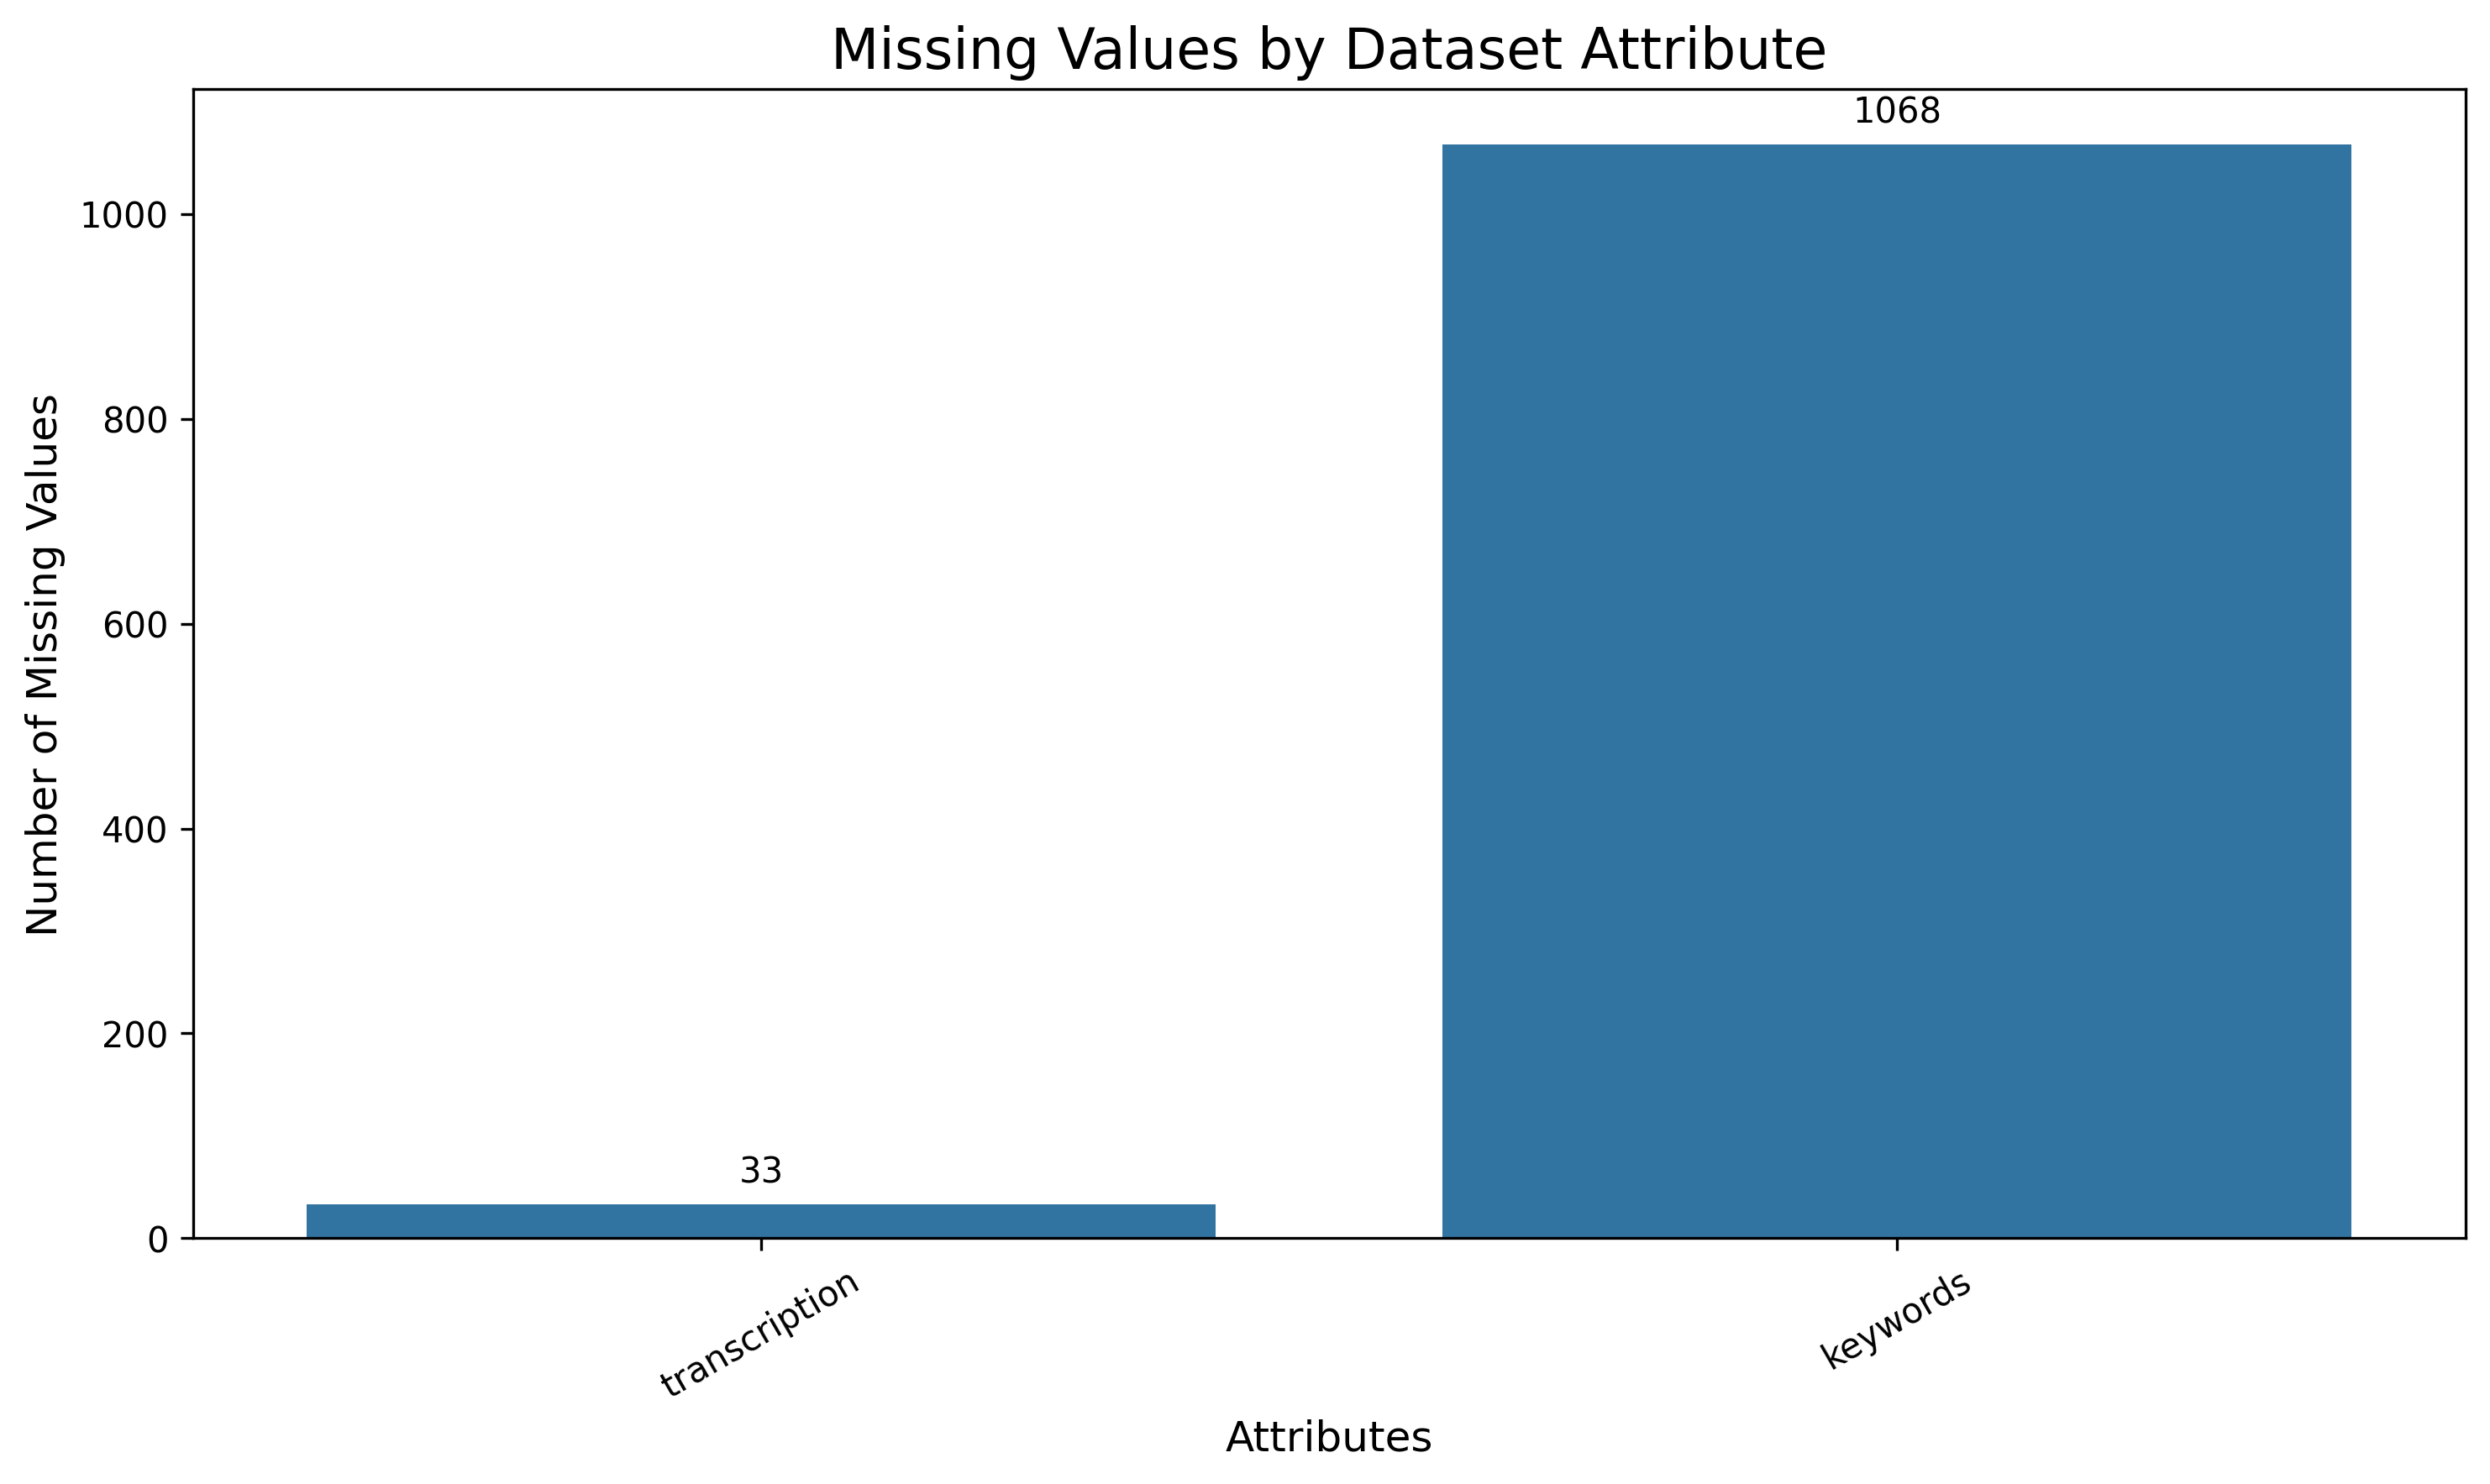
\includegraphics[width=0.82\textwidth,height=6.0cm,keepaspectratio]{EDA_Diagrams/01_missing_values.png}
\caption{Missing Values by Dataset Attribute}
\label{fig:eda_missing}
\end{figure}

\chapter{Top 10 Medical Categories}
Figure \ref{fig:eda_top10} illustrates transcription frequencies for the top 10 categories in the raw dataset. Surgery dominates with 1,103 records, followed by Consult - History and Phy. (516 records), Cardiovascular / Pulmonary (372 records), and Orthopedic (355 records).

\begin{figure}[H]
\centering
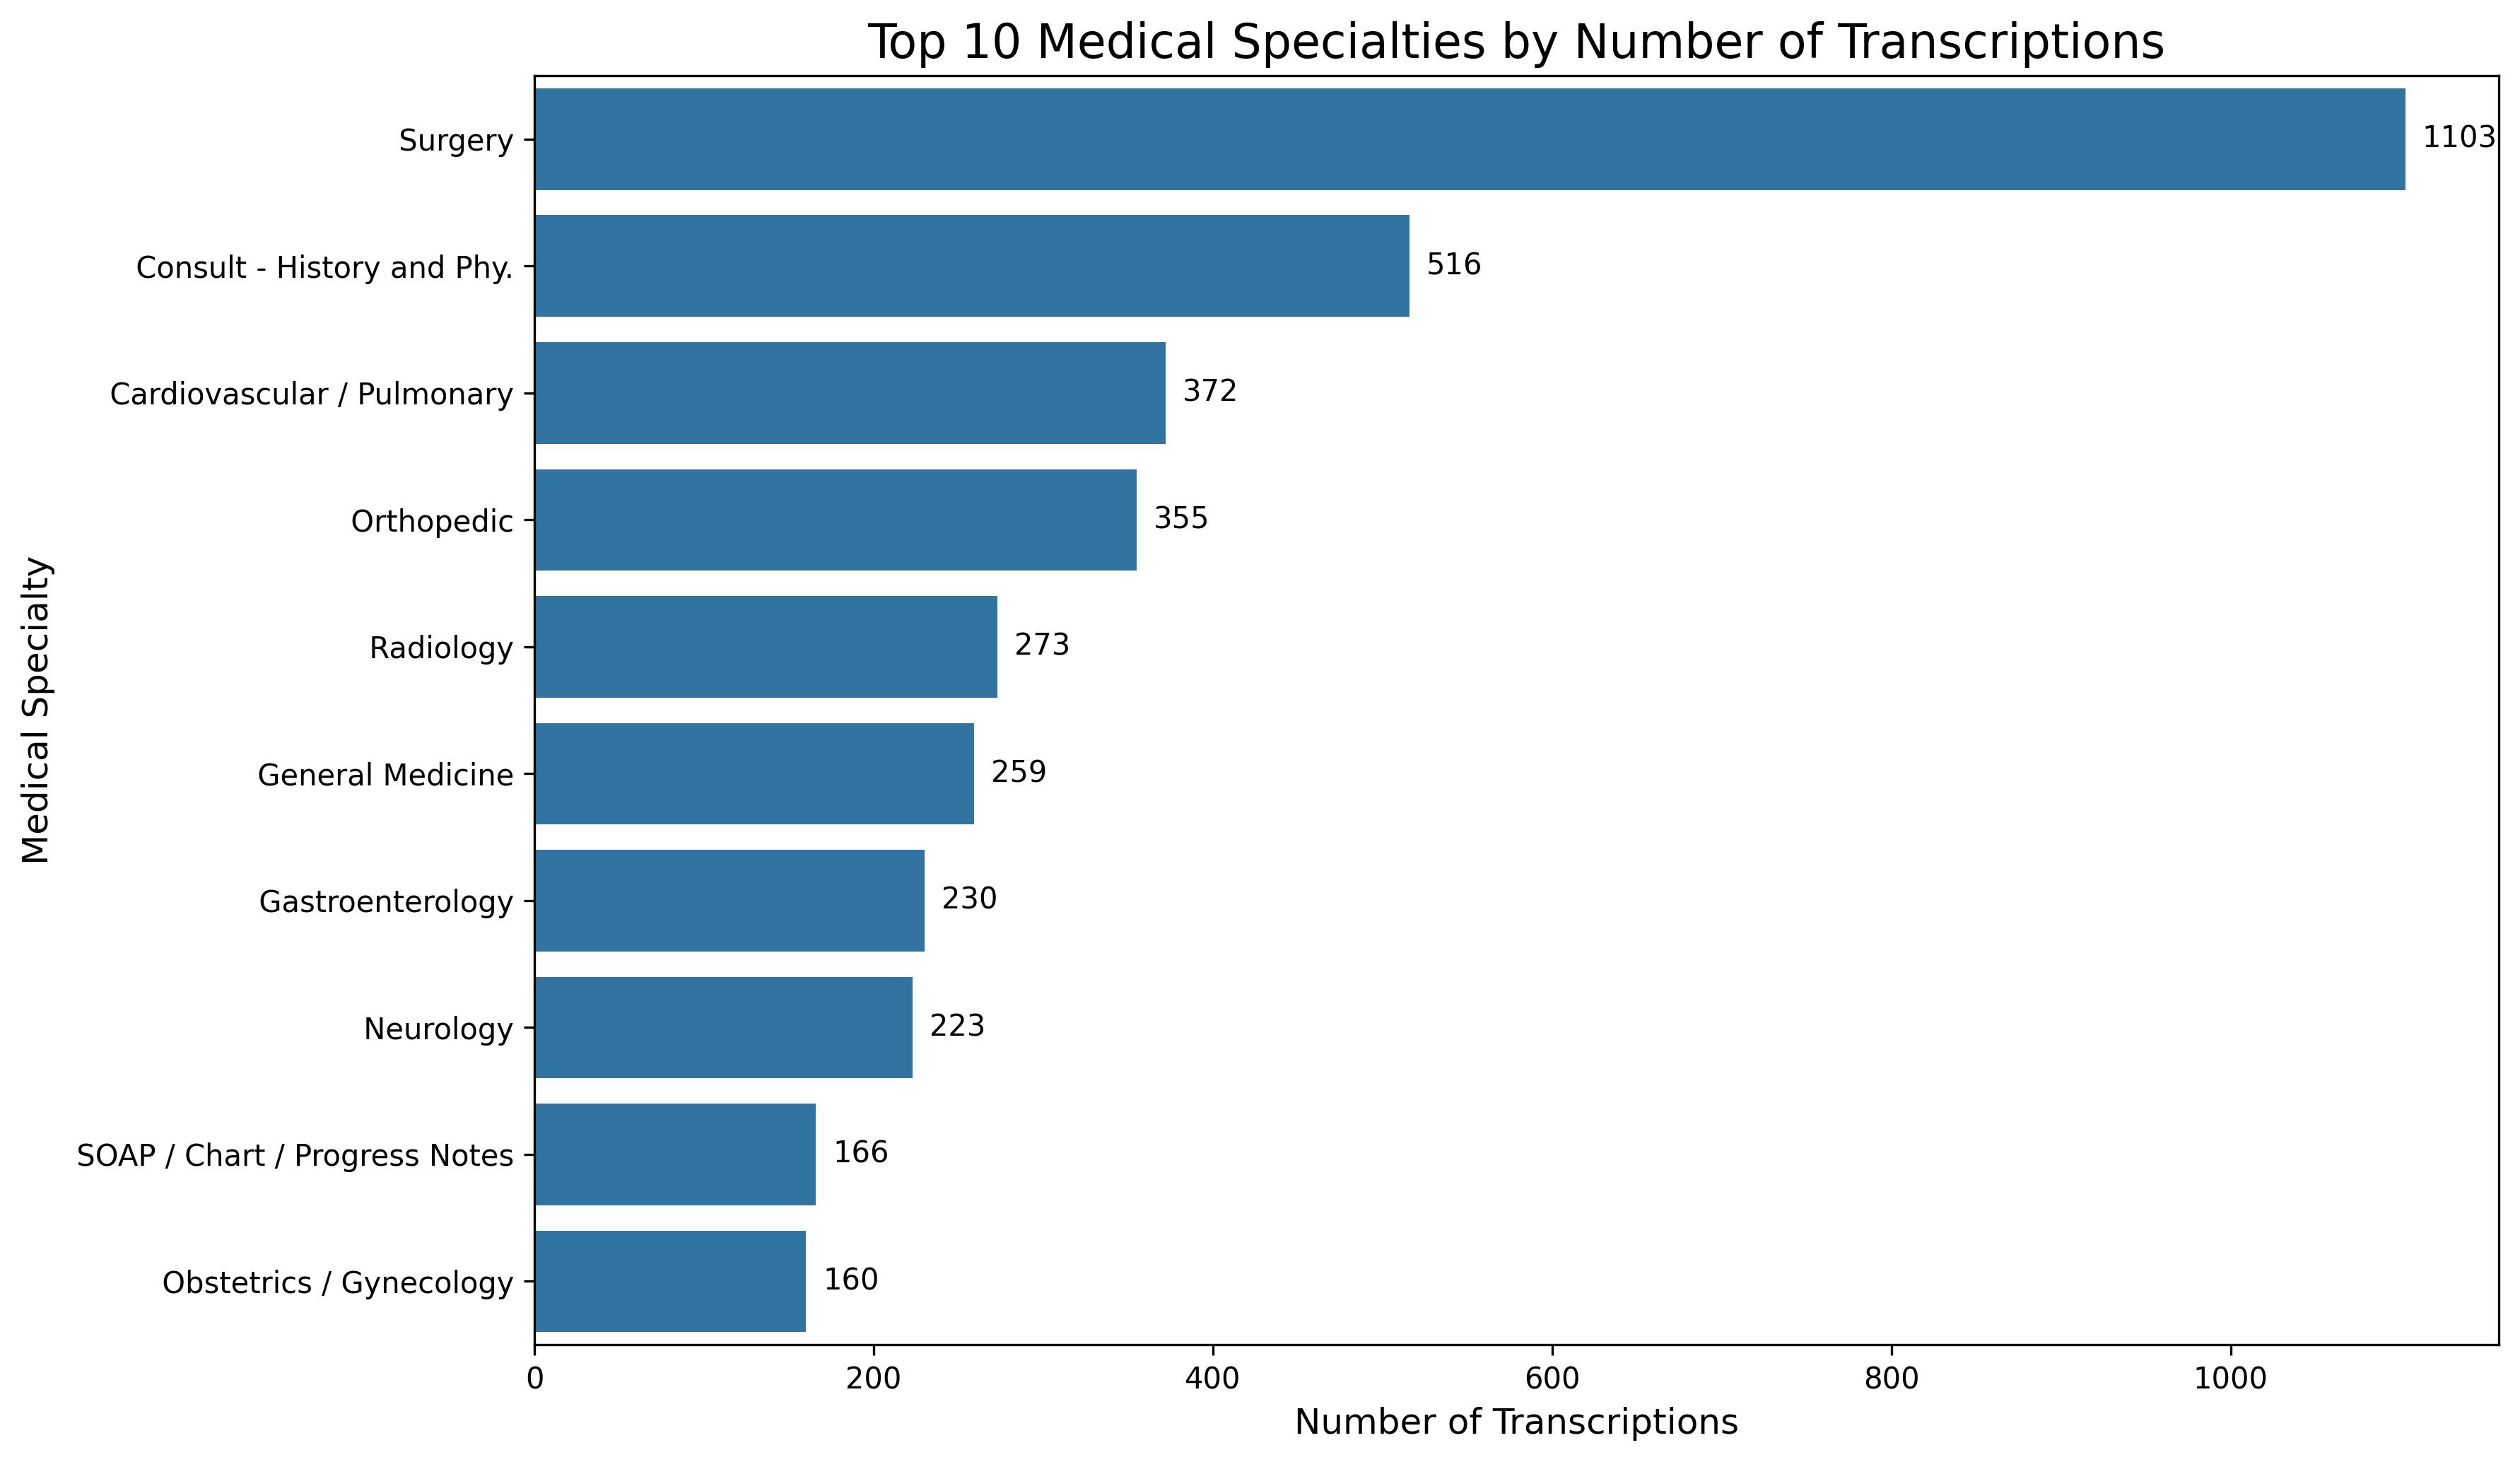
\includegraphics[width=0.82\textwidth,height=6.5cm,keepaspectratio]{EDA_Diagrams/02_top10_medical_specialties.png}
\caption{Top 10 Medical Specialties by Number of Transcriptions}
\label{fig:eda_top10}
\end{figure}

\chapter{Complete Class Distribution (40 Categories)}
Figure \ref{fig:eda_complete_specialty} illustrates the severe class imbalance across all 40 raw categories, underscoring why filtering to 8 mutually exclusive specialties was essential for academic validity.

\begin{figure}[H]
\centering
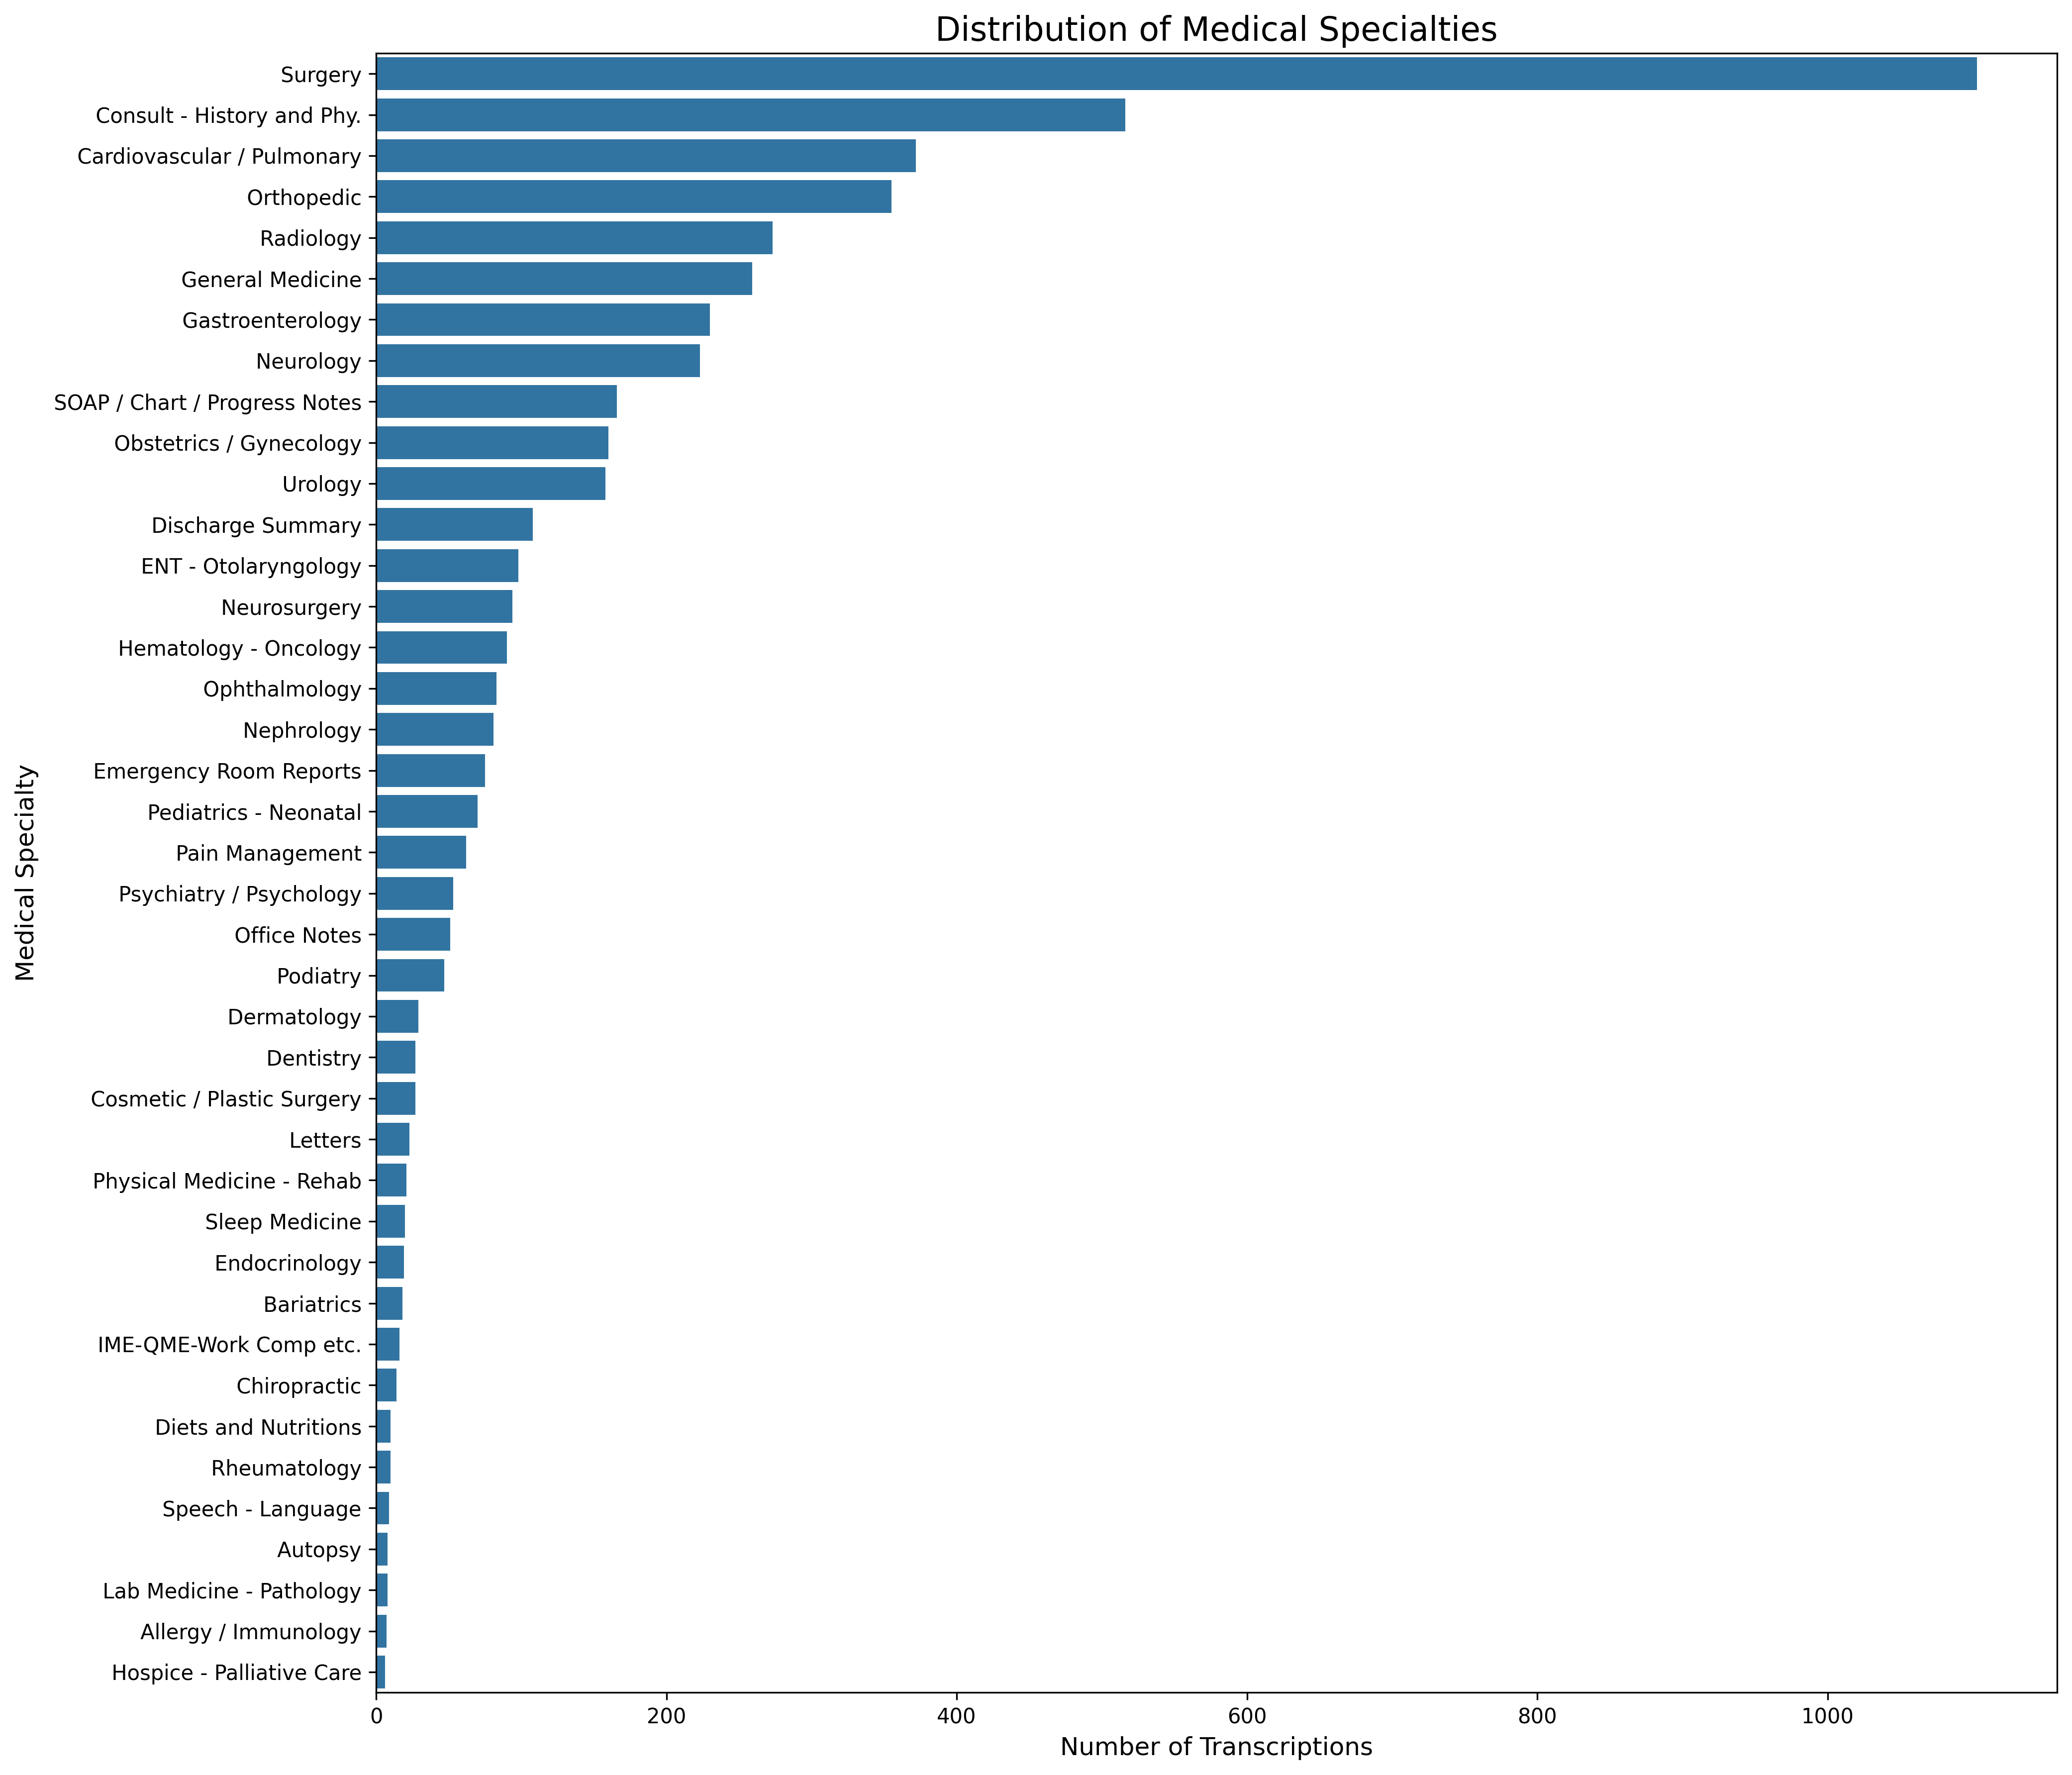
\includegraphics[width=0.82\textwidth,height=7.0cm,keepaspectratio]{EDA_Diagrams/03_complete_specialty_distribution.png}
\caption{Distribution of All 40 Categories in Raw MTSamples Corpus}
\label{fig:eda_complete_specialty}
\end{figure}

\chapter{Clinical Narrative Length Distribution}
Figure \ref{fig:eda_length_dist} displays the word count distribution for clinical narratives, fitted with a Kernel Density Estimate (KDE) curve. The distribution is right-skewed; most transcriptions contain between 200 and 600 words, with comprehensive operative notes extending beyond 2,500 words.

\begin{figure}[H]
\centering
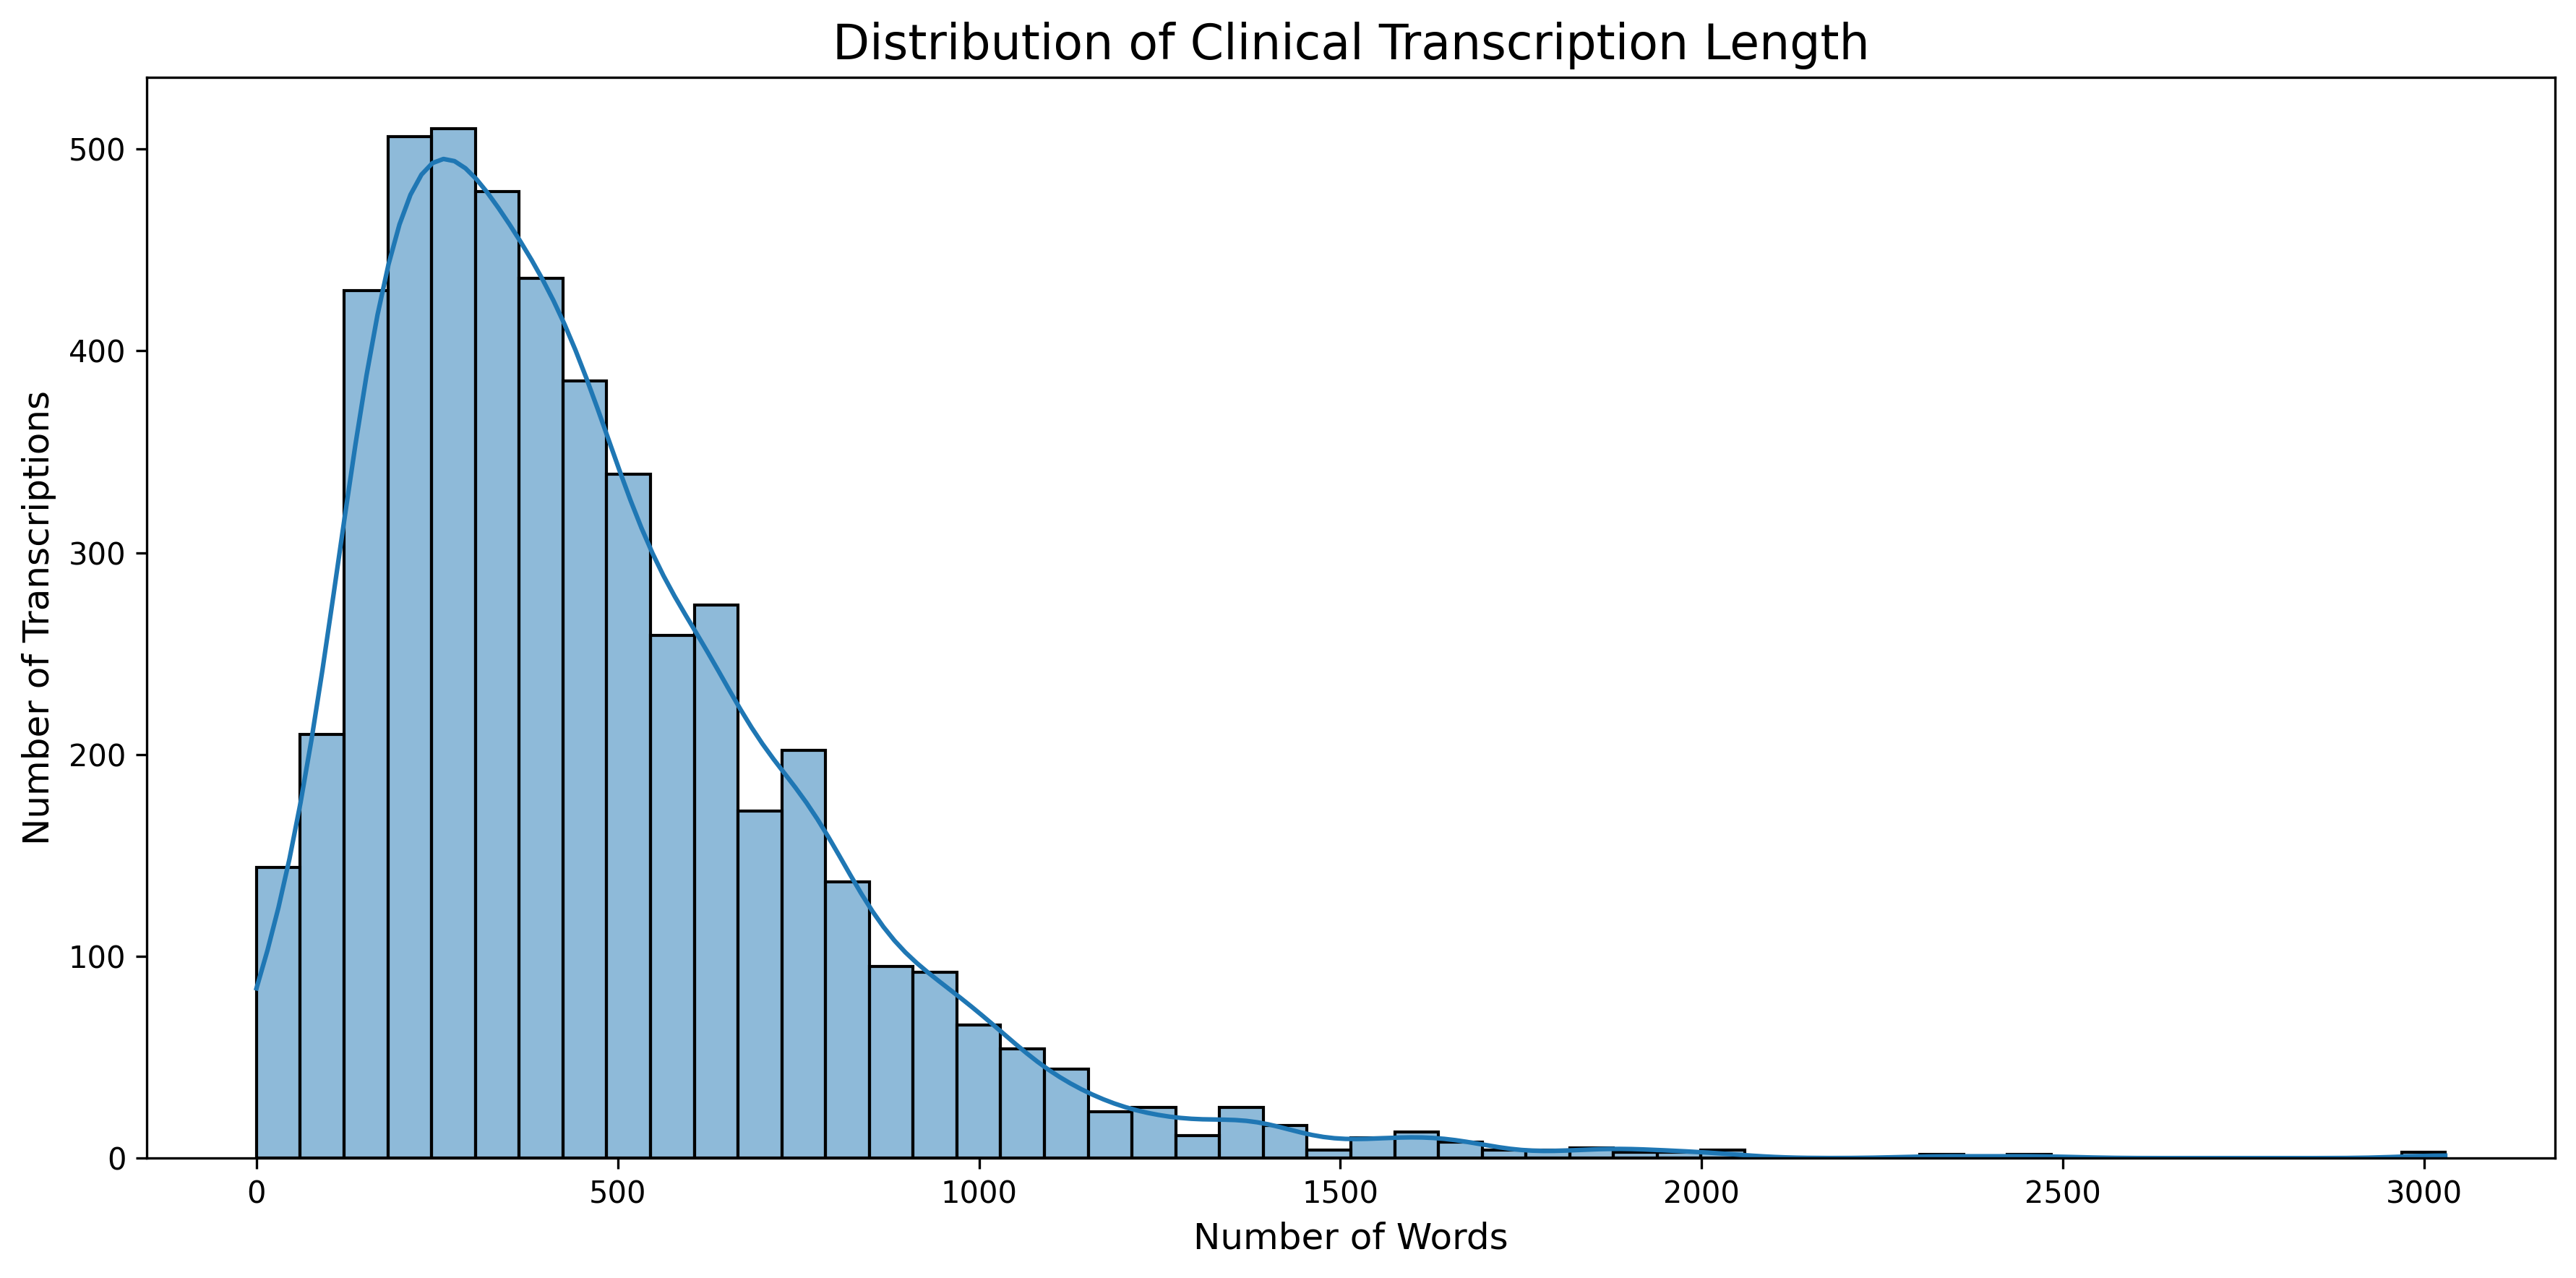
\includegraphics[width=0.82\textwidth,height=6.0cm,keepaspectratio]{EDA_Diagrams/04_transcription_length_distribution.png}
\caption{Distribution of Clinical Transcription Word Length}
\label{fig:eda_length_dist}
\end{figure}

\chapter{Document Length Variations Across Specialties}
Figure \ref{fig:eda_length_by_specialty} presents box plots comparing narrative word count distributions across specialties. Consultations and diagnostic notes (e.g., Radiology) feature shorter median lengths (~200 words), whereas Orthopedic and Cardiovascular operative summaries are substantially longer (~600 words), emphasizing the need for $L_2$ length normalization.

\begin{figure}[H]
\centering
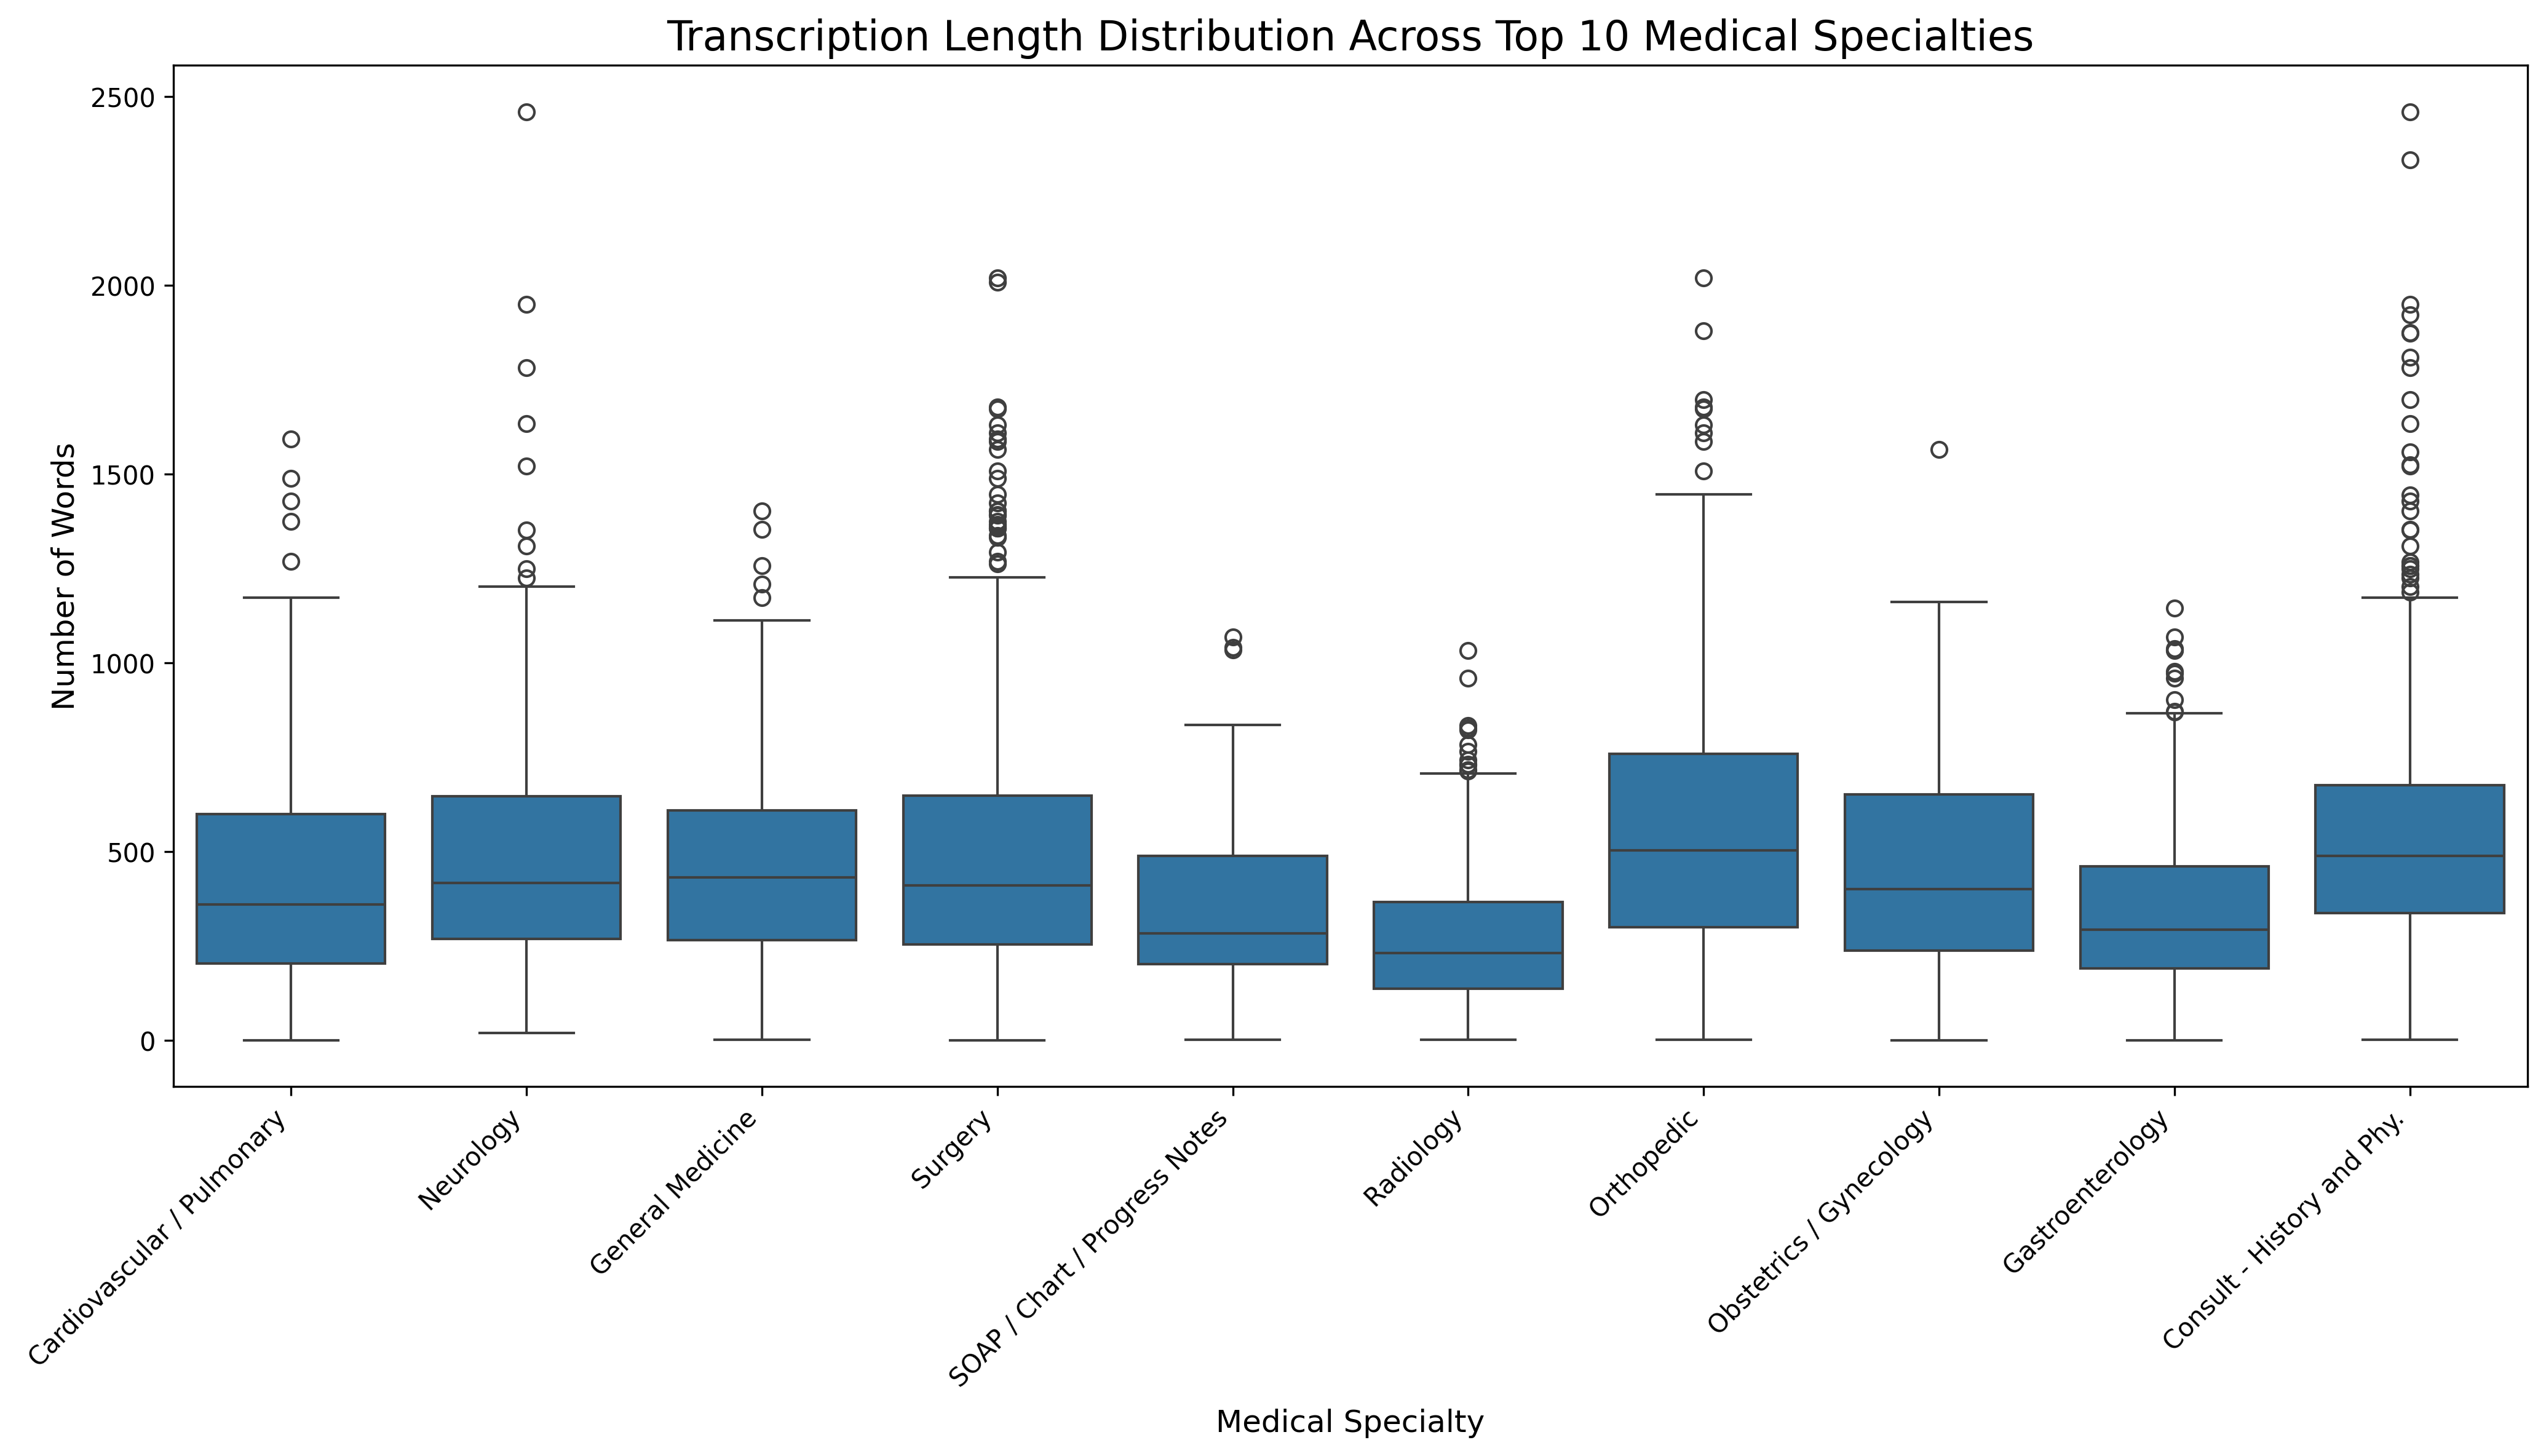
\includegraphics[width=0.82\textwidth,height=6.5cm,keepaspectratio]{EDA_Diagrams/05_transcription_length_by_specialty.png}
\caption{Transcription Length Distribution Across Top Medical Specialties}
\label{fig:eda_length_by_specialty}
\end{figure}

\chapter{Clinical Word Cloud Visualization}
Figure \ref{fig:eda_wordcloud} displays a lexical word cloud of high-frequency clinical terms across the corpus, including ``incision'', ``procedure'', ``patient'', ``normal'', ``placed'', ``artery'', and ``postoperative'', highlighting the medical domain vocabulary.

\begin{figure}[H]
\centering
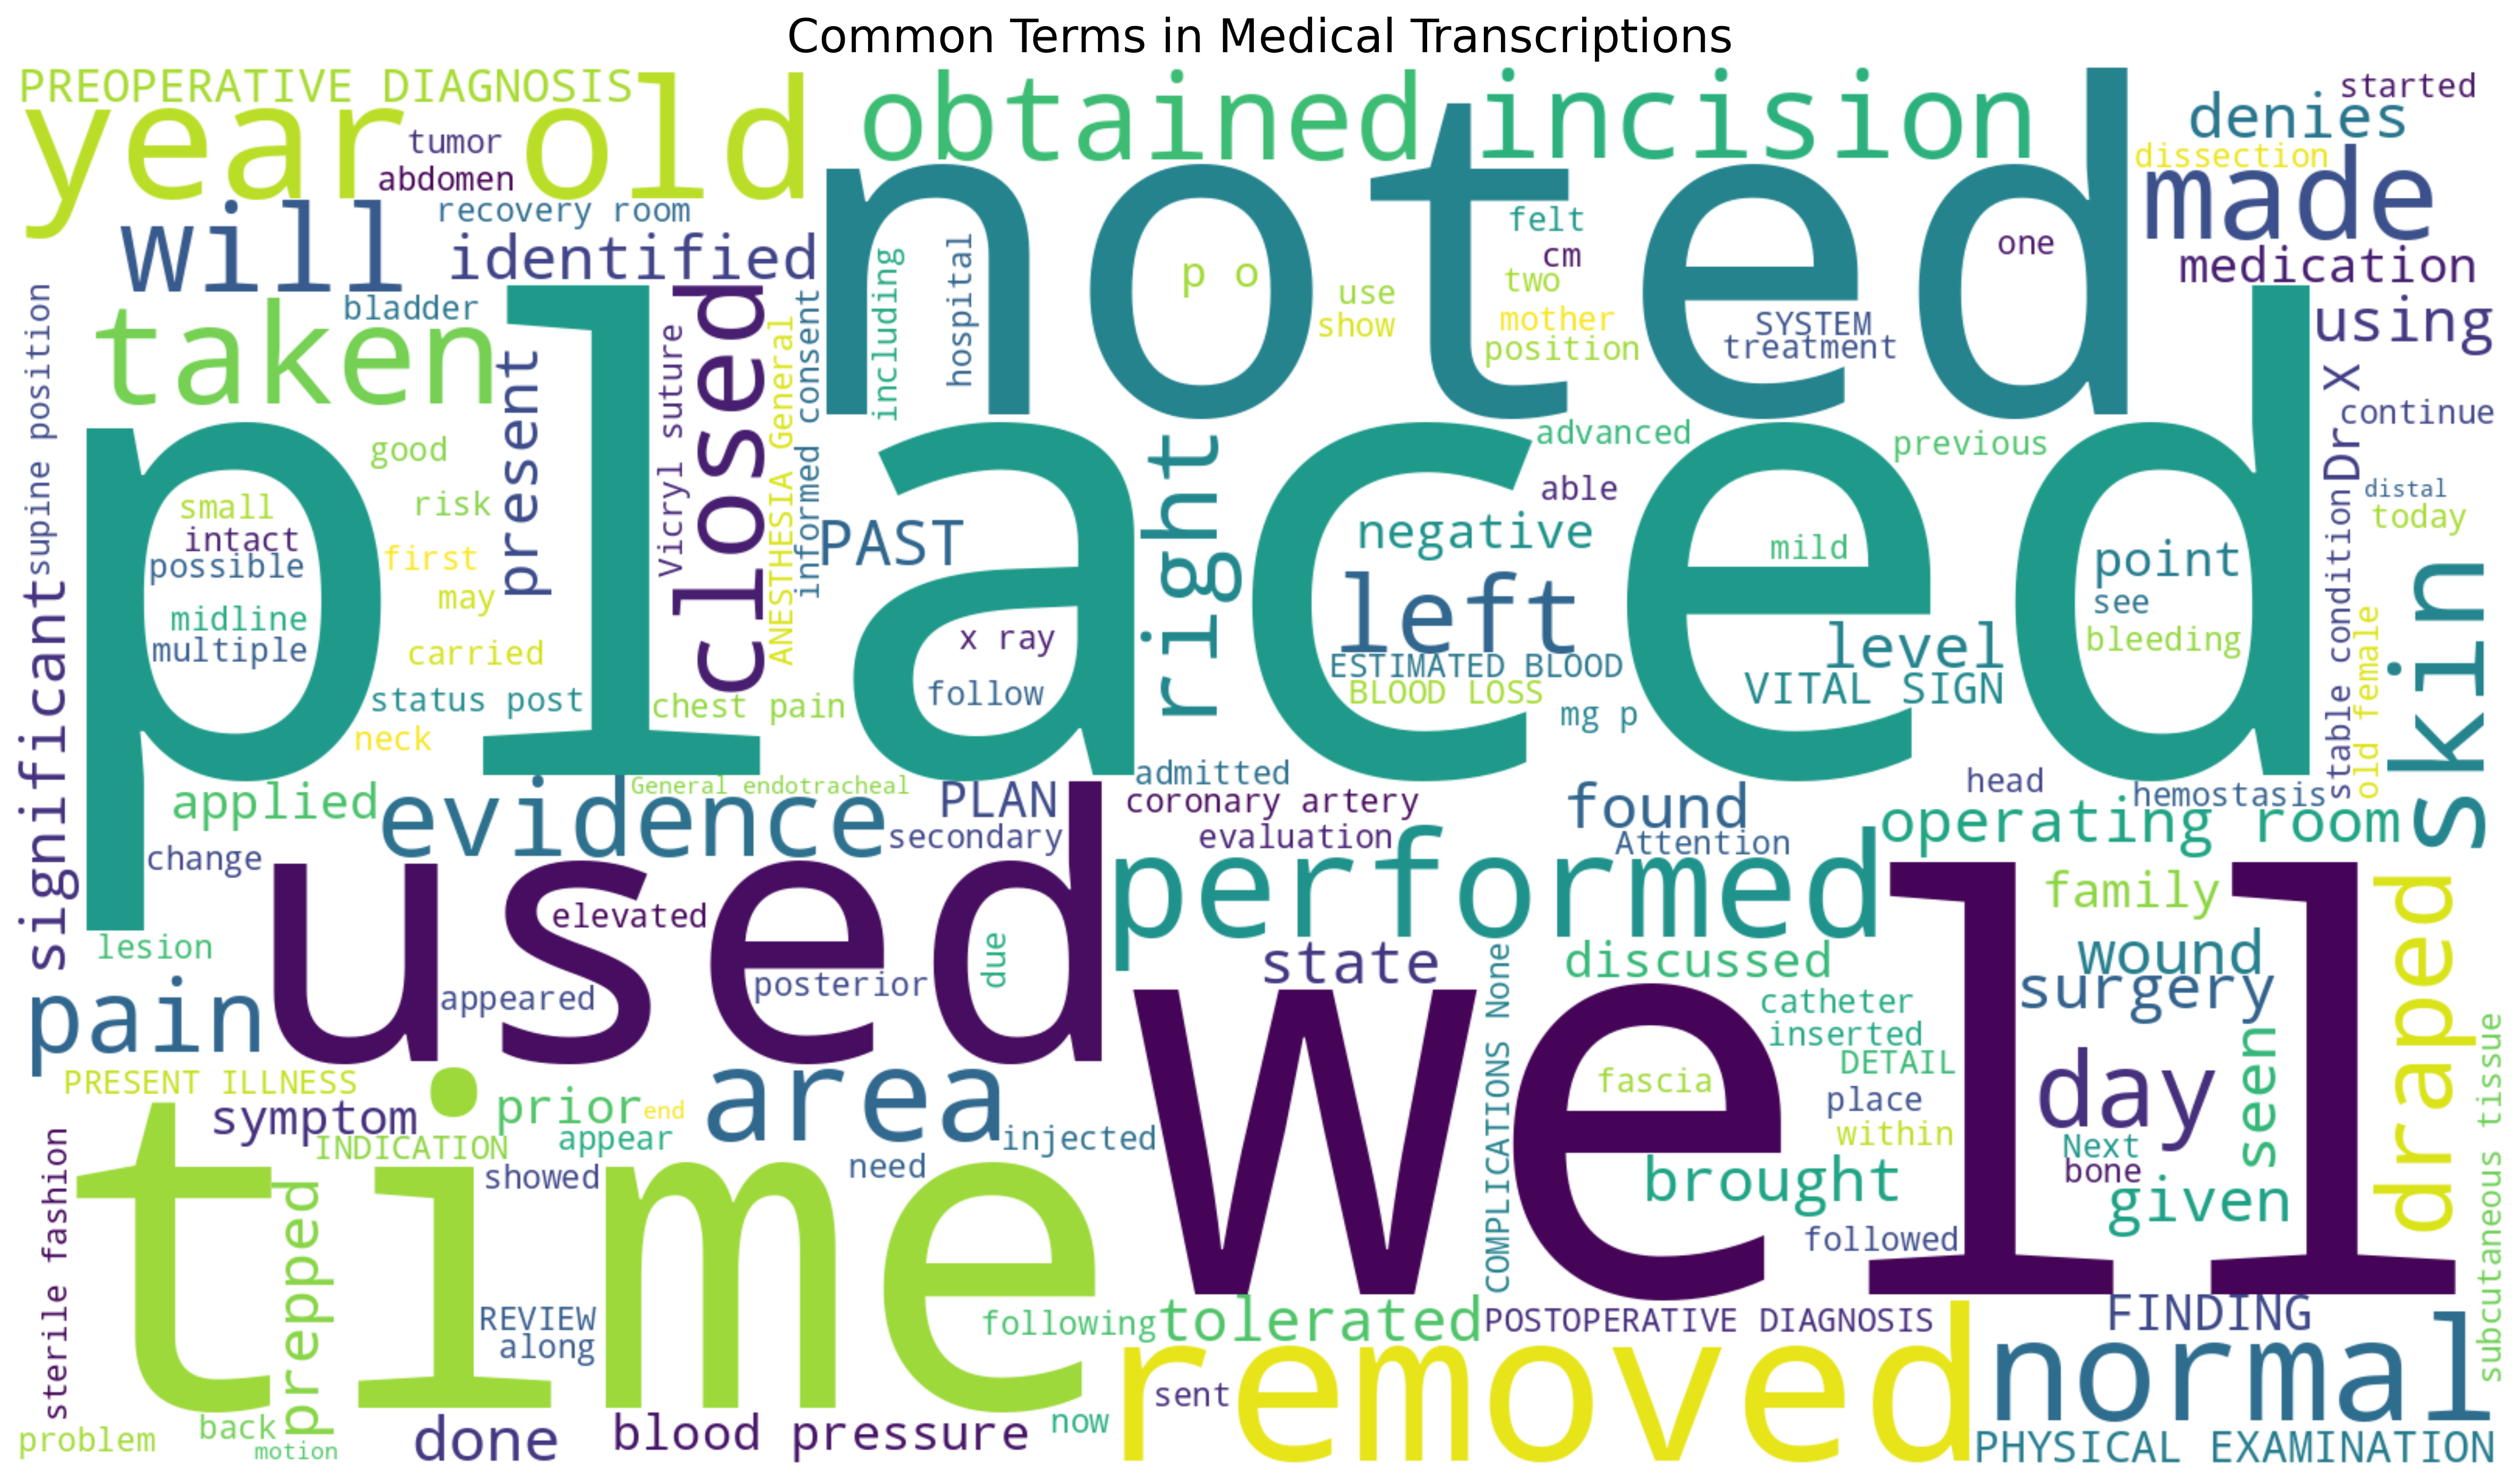
\includegraphics[width=0.82\textwidth,height=6.0cm,keepaspectratio]{EDA_Diagrams/06_medical_transcription_wordcloud.png}
\caption{Common Lexical Terms in Medical Transcriptions}
\label{fig:eda_wordcloud}
\end{figure}

\chapter{Analysis of Architecture and Algorithms}

The classification engine evaluates four candidate supervised learning algorithms alongside sublinear TF-IDF feature extraction, synthesizing their predictions through a calibrated Soft Voting Ensemble with open-set rejection.

\chapter{Detailed Study Report of the Proposed Algorithms}

\chapter{1. Linear Support Vector Machine (Linear SVM)}
Support Vector Machine (SVM) operates on structural risk minimization principles, constructing optimal hyperplanes that maximize the geometric separation margin between clinical classes in high-dimensional feature spaces. Linear SVM is well suited for sparse text categorization where 8,000 TF-IDF features offer natural linear separability.

Given training pairs $(x_i, y_i)$ where $x_i \in \mathbb{R}^d$ and $y_i \in \{1, \dots, K\}$, the soft-margin primal objective is:
\begin{equation}
\min_{w, b, \xi} \frac{1}{2} \|w\|^2 + C \sum_{i=1}^{N} \xi_i
\end{equation}
subject to:
\begin{equation}
y_{i, k}(w_k^T x_i + b_k) \ge 1 - \xi_i, \quad \xi_i \ge 0, \quad \forall i = 1, \dots, N
\end{equation}
where $C$ governs margin trade-offs. To enable soft-voting participation, Linear SVM's uncalibrated signed margin distances $f_k(x) = w_k^T x + b_k$ are calibrated using Scikit-learn's \texttt{CalibratedClassifierCV} via Platt scaling:
\begin{equation}
P_{\text{SVM}}(y = k \mid x) = \frac{1}{1 + \exp(A \cdot f_k(x) + B)}
\end{equation}
mapping geometric margins monotonically into valid multi-class probability distributions.

Figure \ref{fig:act_svm} depicts the activity flow of the Support Vector Machine algorithm.

\begin{figure}[H]
\centering
\begin{tikzpicture}[node distance=0.24cm, auto, >=stealth',
    startstop/.style={rectangle, rounded corners=8pt, draw=black, fill=white, text width=9em, text centered, minimum height=1.5em, font=\scriptsize\bfseries},
    process/.style={rectangle, draw=black, fill=white, text width=14em, text centered, rounded corners=2pt, minimum height=1.5em, font=\scriptsize},
    decision/.style={diamond, draw=black, fill=white, text width=5.5em, text centered, inner sep=0pt, font=\scriptsize},
    branch/.style={rectangle, draw=black, fill=white, text width=7.5em, text centered, rounded corners=2pt, minimum height=1.5em, font=\scriptsize},
    arrow/.style={draw, -latex', semithick}]
    
    \node [startstop] (start) {START};
    \node [process, below=0.24cm of start] (p1) {Input Training TF-IDF Vectors};
    \node [process, below=0.24cm of p1] (p2) {Determine Decision Hyperplanes};
    \node [process, below=0.24cm of p2] (p3) {Calculate Margin ($\frac{2}{\|w\|}$)};
    \node [process, below=0.24cm of p3] (p4) {Identify Critical Support Vectors};
    \node [process, below=0.24cm of p4] (p5) {Optimize Hyperplane and Margin};
    \node [decision, below=0.28cm of p5] (dec1) {Converged?};
    \node [process, below=0.28cm of dec1] (p6) {Calibrate Probabilities (Platt Scaling)};
    \node [process, below=0.24cm of p6] (p7) {Input New Clinical Transcription};
    \node [process, below=0.24cm of p7] (p8) {Compute Calibrated Posteriors $P(y=k|x)$};
    \node [process, below=0.24cm of p8] (p9) {Select Maximum Probability Class};
    \node [branch, below=0.24cm of p9] (out) {Predicted Medical Specialty};
    \node [startstop, below=0.24cm of out] (end) {END};
    
    \path [arrow] (start) -- (p1);
    \path [arrow] (p1) -- (p2);
    \path [arrow] (p2) -- (p3);
    \path [arrow] (p3) -- (p4);
    \path [arrow] (p4) -- (p5);
    \path [arrow] (p5) -- (dec1);
    \path [arrow] (dec1.west) -- node[above, font=\tiny]{No} ([xshift=-0.9cm]p2.west |- dec1.west) -- ([xshift=-0.9cm]p2.west) -- (p2.west);
    \path [arrow] (dec1.south) -- node[right, font=\tiny]{Yes} (p6);
    \path [arrow] (p6) -- (p7);
    \path [arrow] (p7) -- (p8);
    \path [arrow] (p8) -- (p9);
    \path [arrow] (p9) -- (out);
    \path [arrow] (out) -- (end);
\end{tikzpicture}
\caption{Activity Diagram of Support Vector Machine Classifier}
\label{fig:act_svm}
\end{figure}

\chapter{2. Random Forest (RF)}
Random Forest constructs an ensemble of $B = 200$ uncorrelated decision trees using Bootstrap Aggregation (Bagging) paired with random feature subspace selection ($m = \sqrt{d} \approx 89$ features per split). At each internal node, splits minimize Gini Impurity:
\begin{equation}
G = 1 - \sum_{k=1}^{K} p_k^2
\end{equation}
Class probabilities are derived by averaging probability distributions across all trees:
\begin{equation}
P_{\text{RF}}(y = k \mid x) = \frac{1}{B} \sum_{b=1}^{B} P_b(y = k \mid x)
\end{equation}
Random Forest captures complex non-linear keyword interactions that linear boundaries may overlook.

Figure \ref{fig:act_rf} illustrates the operational flow of the Random Forest algorithm.

\begin{figure}[H]
\centering
\begin{tikzpicture}[node distance=0.24cm, auto, >=stealth',
    startstop/.style={rectangle, rounded corners=8pt, draw=black, fill=white, text width=9em, text centered, minimum height=1.5em, font=\scriptsize\bfseries},
    process/.style={rectangle, draw=black, fill=white, text width=14em, text centered, rounded corners=2pt, minimum height=1.5em, font=\scriptsize},
    decision/.style={diamond, draw=black, fill=white, text width=5.5em, text centered, inner sep=0pt, font=\scriptsize},
    branch/.style={rectangle, draw=black, fill=white, text width=7.5em, text centered, rounded corners=2pt, minimum height=1.5em, font=\scriptsize},
    arrow/.style={draw, -latex', semithick}]
    
    \node [startstop] (start) {START};
    \node [process, below=0.24cm of start] (p1) {Input Training TF-IDF Vectors};
    \node [process, below=0.24cm of p1] (p2) {Generate Bootstrap Sample};
    \node [process, below=0.24cm of p2] (p3) {Select Random Feature Subset ($m = \sqrt{d}$)};
    \node [process, below=0.24cm of p3] (p4) {Build Decision Tree via Gini Split};
    \node [decision, below=0.28cm of p4] (dec1) {More Trees?};
    \node [process, below=0.28cm of dec1] (p5) {Forest of Decision Trees Completed};
    \node [process, below=0.24cm of p5] (p6) {Input New Clinical Transcription};
    \node [process, below=0.24cm of p6] (p7) {Obtain Predictions from Each Tree};
    \node [process, below=0.24cm of p7] (p8) {Apply Probability Averaging};
    \node [branch, below=0.24cm of p8] (out) {Predicted Medical Specialty};
    \node [startstop, below=0.24cm of out] (end) {END};
    
    \path [arrow] (start) -- (p1);
    \path [arrow] (p1) -- (p2);
    \path [arrow] (p2) -- (p3);
    \path [arrow] (p3) -- (p4);
    \path [arrow] (p4) -- (dec1);
    \path [arrow] (dec1.west) -- node[above, font=\tiny]{Yes} ([xshift=-0.9cm]p2.west |- dec1.west) -- ([xshift=-0.9cm]p2.west) -- (p2.west);
    \path [arrow] (dec1.south) -- node[right, font=\tiny]{No} (p5);
    \path [arrow] (p5) -- (p6);
    \path [arrow] (p6) -- (p7);
    \path [arrow] (p7) -- (p8);
    \path [arrow] (p8) -- (out);
    \path [arrow] (out) -- (end);
\end{tikzpicture}
\caption{Activity Diagram of Random Forest Classifier}
\label{fig:act_rf}
\end{figure}

\chapter{3. Logistic Regression (LR)}
Multinomial Logistic Regression models multi-class posterior probabilities directly using the Softmax activation function:
\begin{equation}
P_{\text{LR}}(y = k \mid x) = \frac{\exp(w_k^T x + b_k)}{\sum_{j=1}^{K} \exp(w_j^T x + b_j)}
\end{equation}
Parameters are estimated by minimizing categorical cross-entropy loss augmented with an $L_2$ Ridge penalty:
\begin{equation}
J(W, b) = -\frac{1}{N} \sum_{i=1}^{N} \sum_{k=1}^{K} \mathbb{I}(y_i = k) \ln P(y_i = k \mid x_i) + \frac{\lambda}{2} \sum_{k=1}^{K} \|w_k\|_2^2
\end{equation}
Logistic Regression provides intrinsically calibrated class probability distributions and high interpretability through log-odds coefficients.

Figure \ref{fig:act_lr} shows the activity flow of Logistic Regression.

\begin{figure}[H]
\centering
\begin{tikzpicture}[node distance=0.24cm, auto, >=stealth',
    startstop/.style={rectangle, rounded corners=8pt, draw=black, fill=white, text width=9em, text centered, minimum height=1.5em, font=\scriptsize\bfseries},
    process/.style={rectangle, draw=black, fill=white, text width=14em, text centered, rounded corners=2pt, minimum height=1.5em, font=\scriptsize},
    decision/.style={diamond, draw=black, fill=white, text width=5.5em, text centered, inner sep=0pt, font=\scriptsize},
    branch/.style={rectangle, draw=black, fill=white, text width=7.5em, text centered, rounded corners=2pt, minimum height=1.5em, font=\scriptsize},
    arrow/.style={draw, -latex', semithick}]
    
    \node [startstop] (start) {START};
    \node [process, below=0.24cm of start] (p1) {Input Training TF-IDF Vectors};
    \node [process, below=0.24cm of p1] (p2) {Initialize Weights and Biases};
    \node [process, below=0.24cm of p2] (p3) {Calculate Linear Scores $z_k = w_k^T x + b_k$};
    \node [process, below=0.24cm of p3] (p4) {Apply Softmax Activation Function};
    \node [process, below=0.24cm of p4] (p5) {Calculate Cross-Entropy Loss};
    \node [process, below=0.24cm of p5] (p6) {Update Weights via L-BFGS Optimization};
    \node [decision, below=0.28cm of p6] (dec1) {Converged?};
    \node [process, below=0.28cm of dec1] (p7) {Trained Logistic Regression Model};
    \node [process, below=0.24cm of p7] (p8) {Input New Clinical Transcription};
    \node [process, below=0.24cm of p8] (p9) {Calculate Class Probabilities $P(y=k|x)$};
    \node [process, below=0.24cm of p9] (p10) {Select Highest Probability Class};
    \node [branch, below=0.24cm of p10] (out) {Predicted Medical Specialty};
    \node [startstop, below=0.24cm of out] (end) {END};
    
    \path [arrow] (start) -- (p1);
    \path [arrow] (p1) -- (p2);
    \path [arrow] (p2) -- (p3);
    \path [arrow] (p3) -- (p4);
    \path [arrow] (p4) -- (p5);
    \path [arrow] (p5) -- (p6);
    \path [arrow] (p6) -- (dec1);
    \path [arrow] (dec1.west) -- node[above, font=\tiny]{No} ([xshift=-0.9cm]p3.west |- dec1.west) -- ([xshift=-0.9cm]p3.west) -- (p3.west);
    \path [arrow] (dec1.south) -- node[right, font=\tiny]{Yes} (p7);
    \path [arrow] (p7) -- (p8);
    \path [arrow] (p8) -- (p9);
    \path [arrow] (p9) -- (p10);
    \path [arrow] (p10) -- (out);
    \path [arrow] (out) -- (end);
\end{tikzpicture}
\caption{Activity Diagram of Multinomial Logistic Regression Classifier}
\label{fig:act_lr}
\end{figure}

\chapter{4. Multinomial Naive Bayes (MNB)}
Multinomial Naive Bayes is a probabilistic classifier based on Bayes' Theorem under the conditional feature independence assumption:
\begin{equation}
P_{\text{MNB}}(c \mid x) \propto P(c) \prod_{i=1}^{m} P(x_i \mid c)
\end{equation}
Feature likelihoods incorporate Laplace additive smoothing ($\alpha = 1.0$) to avoid zero-probability penalties:
\begin{equation}
P(x_i \mid c) = \frac{N_{ci} + \alpha}{N_c + \alpha |V|}
\end{equation}
MNB provides a fast, linear-time probabilistic baseline that contributes frequency diversity to the ensemble.

Figure \ref{fig:act_mnb} depicts the operational flow of Multinomial Naive Bayes.

\begin{figure}[H]
\centering
\begin{tikzpicture}[node distance=0.24cm, auto, >=stealth',
    startstop/.style={rectangle, rounded corners=8pt, draw=black, fill=white, text width=9em, text centered, minimum height=1.5em, font=\scriptsize\bfseries},
    process/.style={rectangle, draw=black, fill=white, text width=14em, text centered, rounded corners=2pt, minimum height=1.5em, font=\scriptsize},
    branch/.style={rectangle, draw=black, fill=white, text width=7.5em, text centered, rounded corners=2pt, minimum height=1.5em, font=\scriptsize},
    arrow/.style={draw, -latex', semithick}]
    
    \node [startstop] (start) {START};
    \node [process, below=0.24cm of start] (p1) {Input Training TF-IDF Vectors};
    \node [process, below=0.24cm of p1] (p2) {Calculate Prior Probability $P(c)$};
    \node [process, below=0.24cm of p2] (p3) {Compute Term Frequency per Class};
    \node [process, below=0.24cm of p3] (p4) {Apply Additive Laplace Smoothing ($\alpha=1$)};
    \node [process, below=0.24cm of p4] (p5) {Trained Naive Bayes Model};
    \node [process, below=0.24cm of p5] (p6) {Input New Clinical Transcription};
    \node [process, below=0.24cm of p6] (p7) {Apply Bayes' Theorem for Posterior Prob.};
    \node [process, below=0.24cm of p7] (p8) {Select Maximum Probability Class};
    \node [branch, below=0.24cm of p8] (out) {Predicted Medical Specialty};
    \node [startstop, below=0.24cm of out] (end) {END};
    
    \path [arrow] (start) -- (p1);
    \path [arrow] (p1) -- (p2);
    \path [arrow] (p2) -- (p3);
    \path [arrow] (p3) -- (p4);
    \path [arrow] (p4) -- (p5);
    \path [arrow] (p5) -- (p6);
    \path [arrow] (p6) -- (p7);
    \path [arrow] (p7) -- (p8);
    \path [arrow] (p8) -- (out);
    \path [arrow] (out) -- (end);
\end{tikzpicture}
\caption{Activity Diagram of Multinomial Naive Bayes Classifier}
\label{fig:act_mnb}
\end{figure}

\chapter{5. TF-IDF Feature Vectorizer}
The Sublinear TF-IDF Vectorizer calculates composite weights across unigram and bigram tokens:
\begin{equation}
\text{TF-IDF}(t, d, D) = (1 + \log(f_{t, d})) \times \left(\log\left(\frac{1 + |D|}{1 + |\{d \in D : t \in d\}|}\right) + 1\right)
\end{equation}
followed by Euclidean $L_2$ normalization ($v_{\text{norm}} = v / \|v\|_2$). Figure \ref{fig:act_tfidf} outlines the vectorization flow.

\begin{figure}[H]
\centering
\begin{tikzpicture}[node distance=0.24cm, auto, >=stealth',
    startstop/.style={rectangle, rounded corners=8pt, draw=black, fill=white, text width=9em, text centered, minimum height=1.5em, font=\scriptsize\bfseries},
    process/.style={rectangle, draw=black, fill=white, text width=14em, text centered, rounded corners=2pt, minimum height=1.5em, font=\scriptsize},
    arrow/.style={draw, -latex', semithick}]
    
    \node [startstop] (start) {START};
    \node [process, below=0.24cm of start] (p1) {Input Cleaned Text Narratives};
    \node [process, below=0.24cm of p1] (p2) {Tokenize \& Generate N-Grams (1, 2)};
    \node [process, below=0.24cm of p2] (p3) {Compute Sublinear TF ($1 + \log(\text{TF})$)};
    \node [process, below=0.24cm of p3] (p4) {Compute Smoothed IDF Score};
    \node [process, below=0.24cm of p4] (p5) {Calculate Composite TF-IDF Product};
    \node [process, below=0.24cm of p5] (p6) {Apply Euclidean $L_2$ Normalization};
    \node [process, below=0.24cm of p6] (p7) {Construct 8,000-D Sparse Matrix};
    \node [startstop, below=0.24cm of p7] (end) {END};
    
    \path [arrow] (start) -- (p1);
    \path [arrow] (p1) -- (p2);
    \path [arrow] (p2) -- (p3);
    \path [arrow] (p3) -- (p4);
    \path [arrow] (p4) -- (p5);
    \path [arrow] (p5) -- (p6);
    \path [arrow] (p6) -- (p7);
    \path [arrow] (p7) -- (end);
\end{tikzpicture}
\caption{Activity Diagram of Sublinear TF-IDF Feature Vectorizer}
\label{fig:act_tfidf}
\end{figure}

\chapter{6. Soft Voting Ensemble Classifier}
The Soft Voting Ensemble aggregates posterior class probabilities generated by the candidate estimators using calibrated weights $[w_{\text{SVM}}=2, w_{\text{LR}}=2, w_{\text{RF}}=1, w_{\text{MNB}}=1]$:
\begin{equation}
P_{\text{ensemble}}(y = k \mid x) = \frac{2 P_{\text{SVM}}(y = k \mid x) + 2 P_{\text{LR}}(y = k \mid x) + 1 P_{\text{RF}}(y = k \mid x) + 1 P_{\text{MNB}}(y = k \mid x)}{6}
\end{equation}
Linear SVM and Logistic Regression receive double weight due to their superior individual benchmark accuracies (88.59\% and 87.09\%) and strong probability calibration. Random Forest and Naive Bayes contribute architectural non-linearity and probabilistic frequency smoothing with unit weights.

Figure \ref{fig:act_ensemble} displays the architecture and dataflow of the Soft Voting Ensemble Classifier.

\begin{figure}[H]
\centering
\begin{tikzpicture}[node distance=0.35cm and 0.2cm, auto, >=stealth',
    startstop/.style={rectangle, rounded corners=8pt, draw=black, fill=white, text width=9em, text centered, minimum height=1.5em, font=\scriptsize\bfseries},
    process/.style={rectangle, draw=black, fill=white, text width=15em, text centered, rounded corners=2pt, minimum height=1.6em, font=\scriptsize},
    smallbox/.style={rectangle, draw=black, fill=white, text width=6.5em, text centered, rounded corners=2pt, minimum height=2.4em, font=\scriptsize},
    branch/.style={rectangle, draw=black, fill=white, text width=7.5em, text centered, rounded corners=2pt, minimum height=1.5em, font=\scriptsize},
    arrow/.style={draw, -latex', semithick}]
    
    \node [startstop] (start) at (0, 0) {START};
    \node [process, below=0.35cm of start] (input) {TF-IDF Feature Vector Input};
    
    \node [smallbox, below=1.05cm of input, xshift=-4.5cm] (svm) {Linear SVM\\(Weight: 2)};
    \node [smallbox, below=1.05cm of input, xshift=-1.5cm] (lr)  {Logistic Reg.\\(Weight: 2)};
    \node [smallbox, below=1.05cm of input, xshift=1.5cm]  (rf)  {Random Forest\\(Weight: 1)};
    \node [smallbox, below=1.05cm of input, xshift=4.5cm]  (nb)  {Naive Bayes\\(Weight: 1)};
    
    \coordinate (bus1) at ([yshift=-0.52cm]input.south);
    
    \node [process, text width=13cm, below=0.85cm of lr, xshift=1.5cm] (collect) {Collect Calibrated Probabilities Across All Estimators};
    \node [process, below=0.35cm of collect] (vote) {Compute Weighted Soft Voting Consensus: $\sum w_i P_i / 6$};
    \node [process, below=0.35cm of vote] (gate) {Evaluate Open-Set Confidence Gate ($\tau = 0.48$)};
    \node [branch, below=0.35cm of gate] (output) {Specialty Decision / ``Other''};
    \node [startstop, below=0.35cm of output] (end) {END};
    
    \path [arrow] (start) -- (input);
    \path [arrow] (input.south) -- (bus1) -| (svm.north);
    \path [arrow] (input.south) -- (bus1) -| (lr.north);
    \path [arrow] (input.south) -- (bus1) -| (rf.north);
    \path [arrow] (input.south) -- (bus1) -| (nb.north);
    
    \path [arrow] (svm.south) -- ([xshift=-4.5cm]collect.north);
    \path [arrow] (lr.south)  -- ([xshift=-1.5cm]collect.north);
    \path [arrow] (rf.south)  -- ([xshift=1.5cm]collect.north);
    \path [arrow] (nb.south)  -- ([xshift=4.5cm]collect.north);
    
    \path [arrow] (collect) -- (vote);
    \path [arrow] (vote) -- (gate);
    \path [arrow] (gate) -- (output);
    \path [arrow] (output) -- (end);
\end{tikzpicture}
\caption{Activity Diagram of Calibrated Soft Voting Ensemble Classifier}
\label{fig:act_ensemble}
\end{figure}

\chapter{Step-by-Step Working of the Algorithmic Architecture}
The end-to-end classification system executes through nine operational steps:
\begin{enumerate}
    \item \textbf{Clinical Ingestion}: Ingesting patient documentation through PDF upload (PyMuPDF) or manual transcription entry.
    \item \textbf{Text Purification}: Normalizing text, stripping punctuation, converting to lowercase, and handling whitespace.
    \item \textbf{Tokenization \& Stopword Elimination}: Splitting narratives into word tokens and pruning non-informative stopwords.
    \item \textbf{Morphological Lemmatization}: Mapping inflected clinical terms to base WordNet lemmas.
    \item \textbf{Sublinear TF-IDF Vectorization}: Transforming clean text into an 8,000-dimensional sparse feature vector using unigrams and bigrams with $L_2$ normalization.
    \item \textbf{Parallel Classifier Inference}: Concurrently feeding the feature vector to Linear SVM, Logistic Regression, Random Forest, and Multinomial Naive Bayes to generate posterior probability distributions.
    \item \textbf{Weighted Soft Voting Consensus}: Calculating aggregated posterior class probabilities using calibrated weights $[2, 2, 1, 1]$.
    \item \textbf{Open-Set Confidence Check ($\tau = 0.48$)}: If the peak ensemble probability is $\ge 0.48$, confirming the predicted medical specialty; otherwise, routing the report to \textit{``Other / Requires Review''}.
    \item \textbf{Decision Output \& UI Visualization}: Presenting the specialty decision, probability distribution bars, telemetry metrics, and top candidate domains in the web application.
\end{enumerate}

\chapter{Project pipeline}

The project pipeline structures the end-to-end transformation of clinical text from raw data ingestion to interactive web deployment without test-set data leakage. Figure \ref{fig:project_pipeline} illustrates the complete pipeline dataflow.

\begin{figure}[H]
\centering
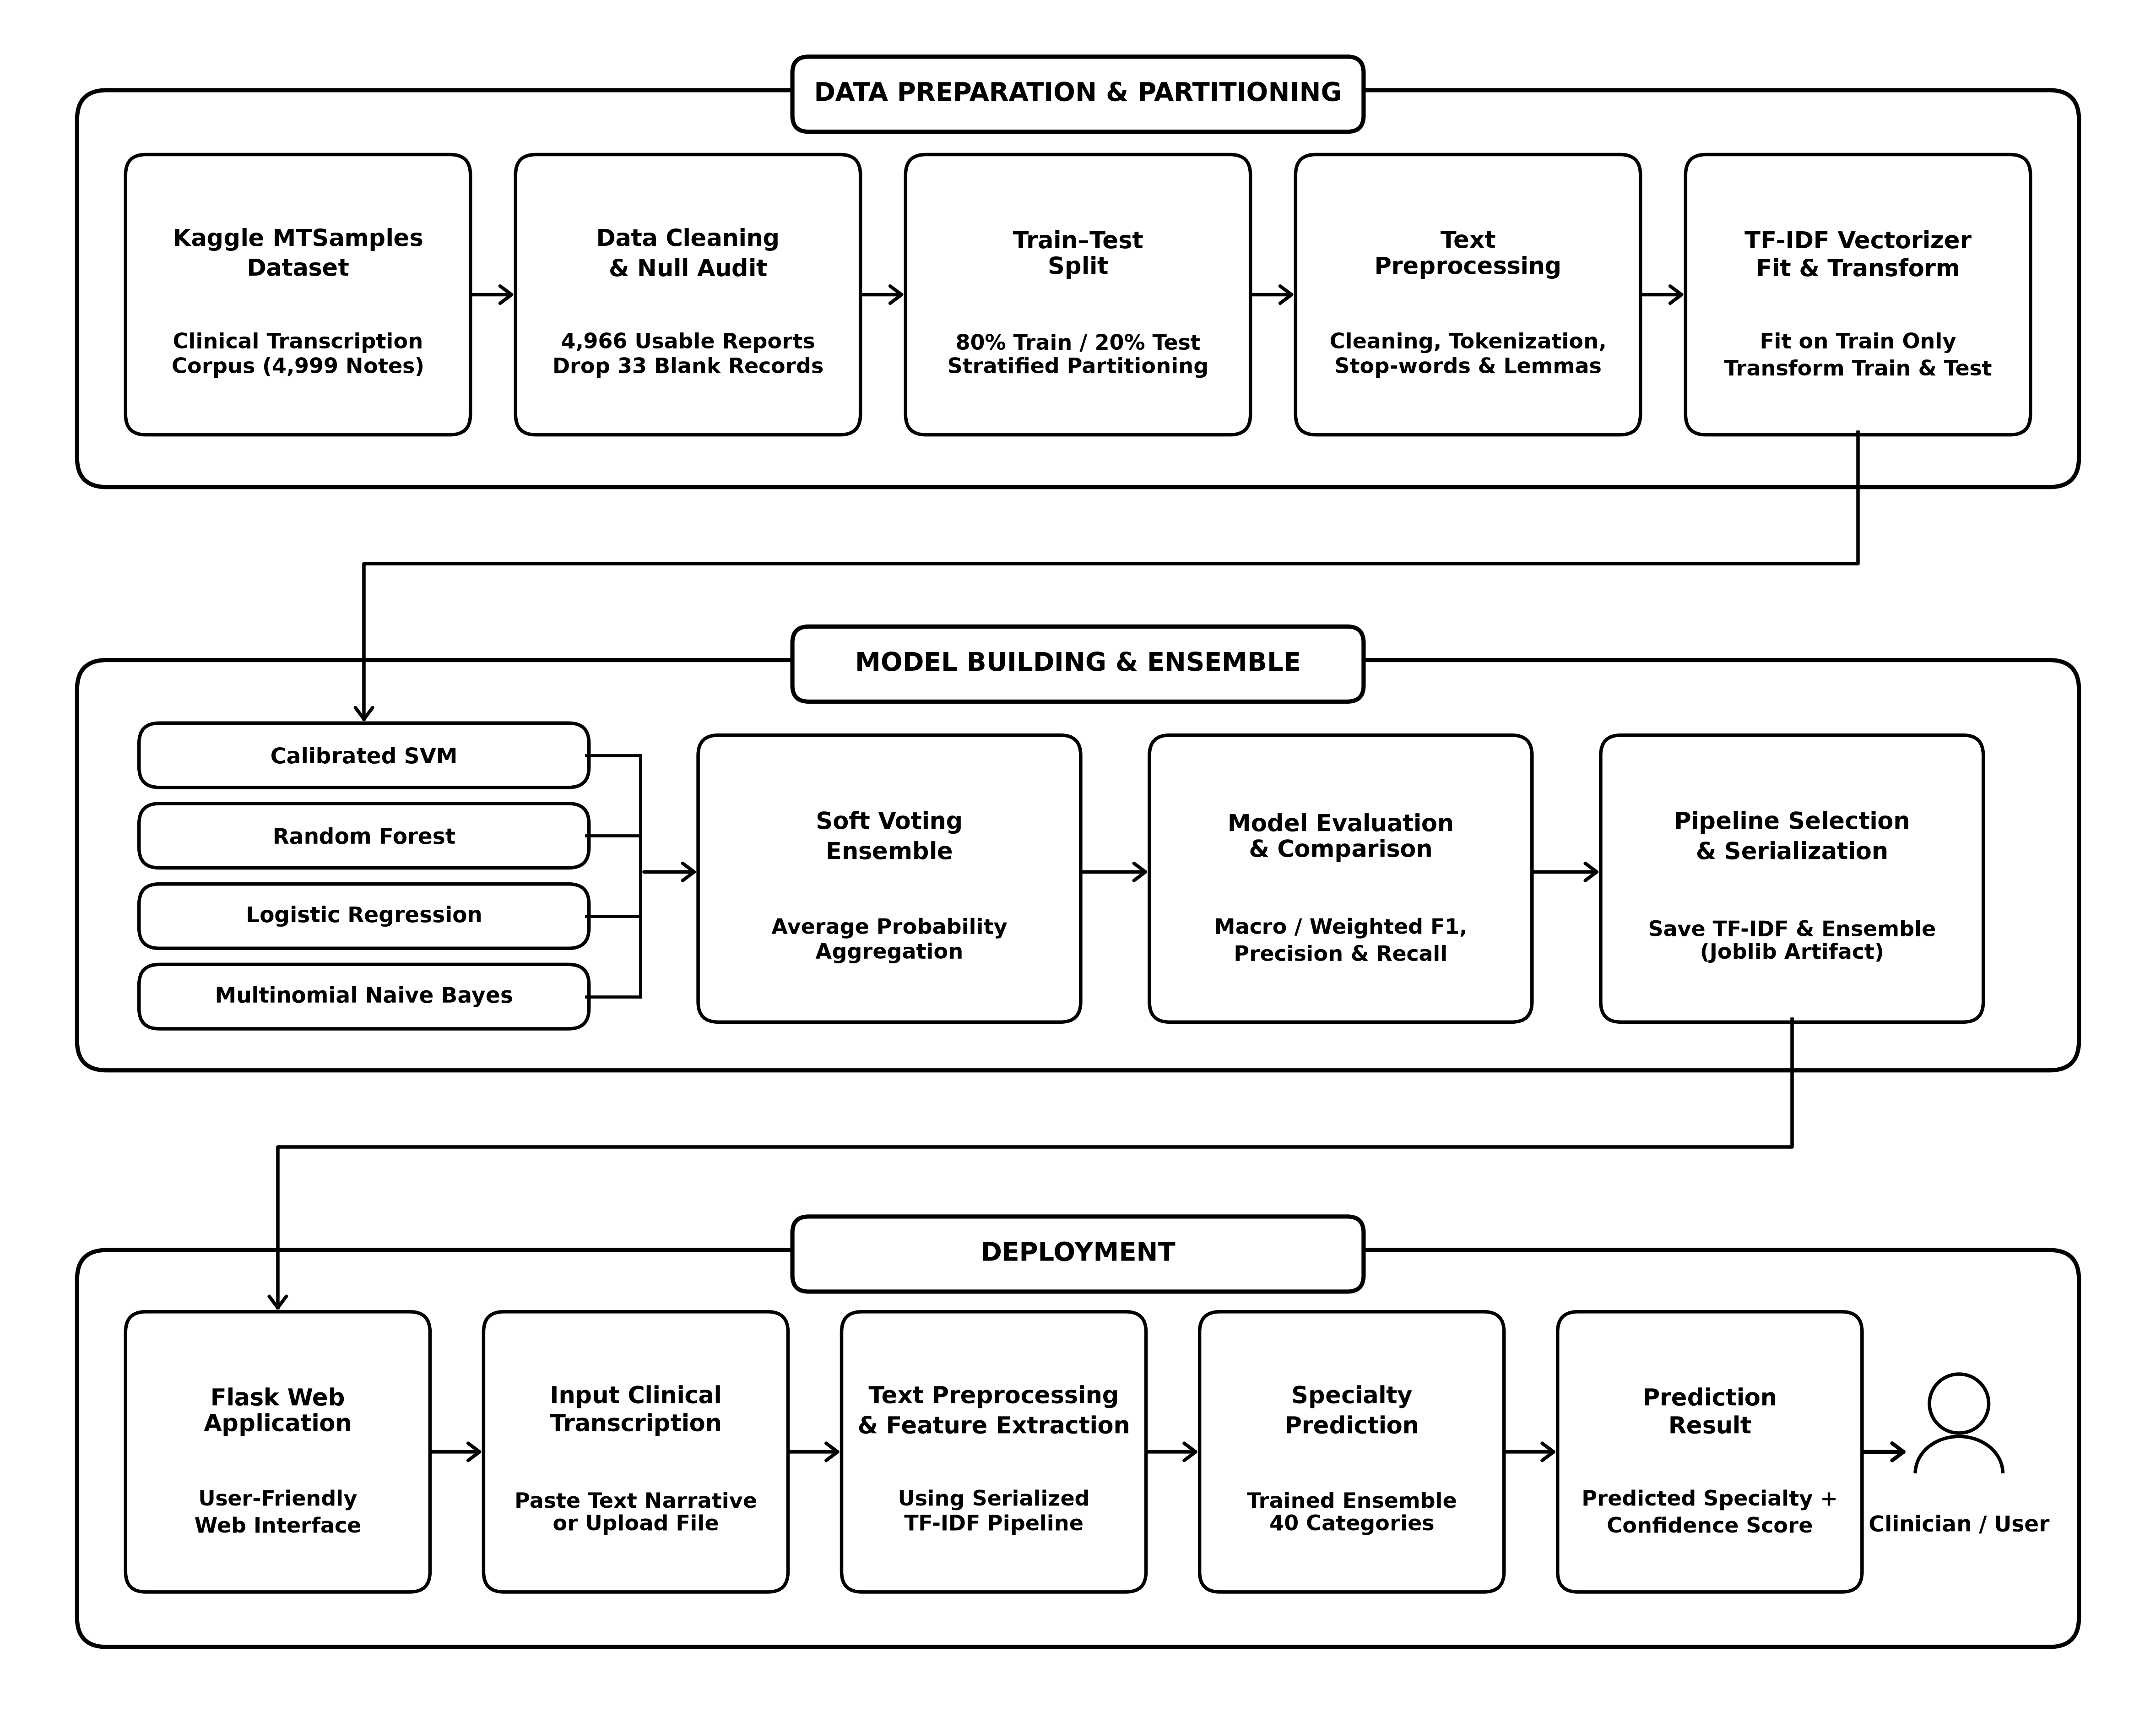
\includegraphics[width=\linewidth]{EDA_Diagrams/07_project_pipeline.png}
\caption{Project Pipeline Diagram of Medical Specialty Classification System}
\label{fig:project_pipeline}
\end{figure}

The pipeline is organized into twelve sequential operational levels:
\begin{enumerate}
    \item \textbf{Data Acquisition}: Ingesting raw MTSamples clinical records (4,999 records).
    \item \textbf{Domain Curation}: Pruning administrative templates and filtering to the 8 core mutually exclusive hospital specialties (1,663 records).
    \item \textbf{Exploratory Profiling}: Conducting statistical audits of text length distributions, class frequencies, and missing values.
    \item \textbf{Stratified Train-Test Splitting}: Partitioning the curated dataset into an 80\% training partition (1,330 records) and a 20\% testing partition (333 records) using stratified sampling prior to vectorization to strictly prevent data leakage.
    \item \textbf{NLP Preprocessing}: Executing text cleaning, tokenization, stopword removal, and morphological lemmatization on both partitions.
    \item \textbf{TF-IDF Vectorizer Fitting}: Fitting the 8,000-feature sublinear TF-IDF vectorizer exclusively on the training partition and transforming both splits into normalized sparse matrices.
    \item \textbf{Base Classifier Training}: Fitting Linear SVM, Logistic Regression, Random Forest, and Multinomial Naive Bayes on training features.
    \item \textbf{Probability Calibration}: Calibrating Linear SVM margin scores using Platt scaling (\texttt{CalibratedClassifierCV}).
    \item \textbf{Soft Voting Ensemble Formulation}: Aggregating base model probabilities using calibrated weights [2:2:1:1].
    \item \textbf{Open-Set Confidence Gate}: Applying safety threshold $\tau = 0.48$ to triage ambiguous or out-of-scope records to ``Other''.
    \item \textbf{Empirical Multi-Metric Evaluation}: Evaluating holdout test set performance using Accuracy, Macro F1, Confusion Matrix, and Precision/Recall reports.
    \item \textbf{Pipeline Serialization \& Web Deployment}: Serializing artifacts with Joblib and deploying the MedSpecialty AI Platform web application with PyMuPDF PDF extraction.
\end{enumerate}

\FloatBarrier

\chapter{Project Timeline}
Table \ref{tab:project_timeline} details the project timeline, milestones, and sprint releases.

\begin{table}[H]
\centering
\small
\renewcommand{\arraystretch}{1.06}
\setlength{\tabcolsep}{6pt}
\begin{tabularx}{\linewidth}{|>{\raggedright\arraybackslash}p{3.8cm}|>{\raggedright\arraybackslash}X|}
\hline
\textbf{Period / Date} & \textbf{Planned Activity} \\
\hline
17.07.2026 & Project Proposal \& Synopsis Approval by Guide \\
\hline
20.07.2026 -- 21.07.2026 & Project Proposal Presentation before Approval Committee \\
\hline
Week 1--2 & Dataset Collection, Null Audit, and Initial EDA \\
\hline
Week 3--4 & Clinical Domain Filtering (8 Core Classes) and Text Preprocessing \\
\hline
Week 5 & Sublinear TF-IDF Feature Extraction \& Vectorization (8,000 Dimensions) \\
\hline
08.09.2026 & First Project Presentation (Phase 1 Faculty Review) \\
\hline
09.09.2026 & Sprint Release I (Dataset Exploration \& NLP Preprocessing) \\
\hline
Week 6 & Candidate ML Model Training (Linear SVM, RF, LR, MNB) \\
\hline
18.09.2026 & Sprint Release II \\
\hline
Week 7 & Platt Probability Calibration and Model Evaluation \\
\hline
Week 8 & Soft Voting Ensemble Formulation [2:2:1:1] and Open-Set Rejection Gate \\
\hline
29.09.2026 -- 30.09.2026 & Interim Project Presentation \\
\hline
Week 9 & Flask Web Integration \& MedSpecialty AI Platform Deployment (Stitch UI) \\
\hline
09.10.2026 & Sprint Release III (PDF Ingestion \& End-to-End Testing) \\
\hline
Week 10--11 & Holdout Evaluation, Confusion Matrix Analysis, and Final Report Preparation \\
\hline
22.10.2026 -- 23.10.2026 & Final Project Presentation \\
\hline
30.10.2026 & Final Report Submission \\
\hline
\end{tabularx}
\caption{Project Timeline and Milestone Schedule}
\label{tab:project_timeline}
\end{table}

\FloatBarrier

\chapter{Feasibility Analysis}

Feasibility analysis evaluates the viability of the proposed system across technical, economic, operational, and schedule dimensions.

\chapter{Technical Feasibility}
The system is technically feasible because it is constructed using mature, open-source Python natural language processing and machine learning libraries (Scikit-learn, PyMuPDF, Pandas, NumPy). Classical supervised estimators paired with sublinear TF-IDF vectorization execute with high computational efficiency, eliminating the need for expensive GPU clusters. The model executes inference in under 40 milliseconds on standard CPU hardware, making it well suited for interactive web deployment via the Flask WSGI microframework.

\chapter{Economic Feasibility}
The system is economically feasible as it incurs zero software licensing costs. The MTSamples dataset is publicly accessible, and all software frameworks (Python, Flask, Scikit-learn, PyMuPDF) are free and open-source. Eliminating dedicated cloud GPU instances minimizes operational hosting expenditures, enabling cost-effective deployment on standard institutional servers.

\chapter{Operational Feasibility}
The system is operationally feasible because it provides an intuitive, clinical-grade user interface (\textbf{MedSpecialty AI Platform}) adhering to the Google Stitch design system. Clinicians can drag and drop clinical PDF reports or paste dictated narratives, inspect intermediate NLP pipeline stages, view consensus confidence meters, and receive safe open-set triage recommendations. The workflow integrates seamlessly into hospital health information management routines.

\chapter{Schedule Feasibility}
The project is schedule feasible because all phases---dataset curation, NLP preprocessing, model training, probability calibration, soft voting integration, open-set thresholding, and web deployment---have been completed in alignment with the academic timeline.

\chapter{System Environment}

The system environment defines the software frameworks and hardware configurations utilized for development, evaluation, and deployment.

\chapter{Software Environment}
Table \ref{tab:software_environment} outlines the software tools, frameworks, and their respective operational roles.

\begin{table}[H]
\centering
\small
\renewcommand{\arraystretch}{1.15}
\setlength{\tabcolsep}{5pt}
\begin{tabularx}{\linewidth}{|>{\raggedright\arraybackslash}p{3.2cm}|>{\raggedright\arraybackslash}p{3.0cm}|>{\raggedright\arraybackslash}X|}
\hline
\textbf{Software / Tool} & \textbf{Type} & \textbf{Purpose in System} \\
\hline
Python 3.10+ & Programming Language & Core language for text preprocessing, feature engineering, model training, and API server. \\
\hline
Visual Studio Code & Development IDE & Primary IDE for modular Python script development, project organization, and debugging. \\
\hline
Flask & Web Framework & Lightweight WSGI framework serving REST APIs and hosting the MedSpecialty AI Platform. \\
\hline
PyMuPDF (fitz) & Document Parser & High-speed in-memory PDF text extraction engine for clinical document parsing. \\
\hline
Scikit-learn & Machine Learning & Sublinear TF-IDF vectorizer, candidate classifiers (Linear SVM, LR, RF, MNB), calibration, and voting ensemble. \\
\hline
Joblib & Object Serialization & Serializing trained TF-IDF vectorizer and voting ensemble models for instant loading. \\
\hline
Pandas & Data Manipulation & Ingestion, null audits, domain filtering, and tabular metrics calculation. \\
\hline
NumPy & Numerical Computing & Multi-dimensional array operations and probability tensor calculations. \\
\hline
Matplotlib \& Seaborn & Data Visualization & Generating statistical charts, class distribution plots, and confusion matrix heatmaps. \\
\hline
\LaTeX & Typesetting System & Preparing formatted academic reports and mathematical documentation. \\
\hline
\end{tabularx}
\caption{Software Environment and Tool Specifications}
\label{tab:software_environment}
\end{table}

\FloatBarrier

\chapter{Hardware Environment}
Table \ref{tab:hardware_environment} details the minimum and recommended hardware specifications for developing and hosting the system. The architecture operates entirely on CPU hardware without requiring dedicated GPUs.

\begin{table}[H]
\centering
\small
\renewcommand{\arraystretch}{1.15}
\setlength{\tabcolsep}{5pt}
\begin{tabularx}{\linewidth}{|>{\raggedright\arraybackslash}p{3.5cm}|>{\raggedright\arraybackslash}p{4.2cm}|>{\raggedright\arraybackslash}X|}
\hline
\textbf{Hardware Component} & \textbf{Minimum Requirement} & \textbf{Recommended Specification} \\
\hline
Processor (CPU) & Dual-Core Processor (2.0 GHz or higher) & Quad-Core / Octa-Core Intel Core i5/i7 or AMD Ryzen 5/7 (Multi-core CPU; no GPU required) \\
\hline
RAM & 8 GB DDR4 & 16 GB DDR4/DDR5 (Supports parallel model training and web server handling) \\
\hline
Storage & 20 GB available disk space & 256 GB / 512 GB Solid State Drive (SSD) for rapid dataset read/write and virtual environments \\
\hline
Operating System & Windows 10 (64-bit) & Windows 10/11 (64-bit) or Ubuntu Linux 20.04+ LTS \\
\hline
Display Resolution & $1366 \times 768$ pixels & $1920 \times 1080$ (Full HD) for responsive web UI visualization \\
\hline
\end{tabularx}
\caption{Hardware Specifications and Environment Requirements}
\label{tab:hardware_environment}
\end{table}
